\section{Experiment 3 : DNS}
% Experiment 3-1
\subsection{DNS : Traing DNS with Wireshark \#1}
    % \subsubsection*{Problems}
    \begin{enumerate}[label=\bfseries Problem \arabic*:,leftmargin=*,labelindent=1em]
    % \addtocounter{enumi}{11}
        \item Locate the DNS query and response messages. Are then sent over UDP or TCP?\\[0.2mm]
            \soln User Datagram Protocol (UDP)
            \vspace{-2mm}  
            \begin{figure}[!h]\centering
            \hspace{10mm} 
        		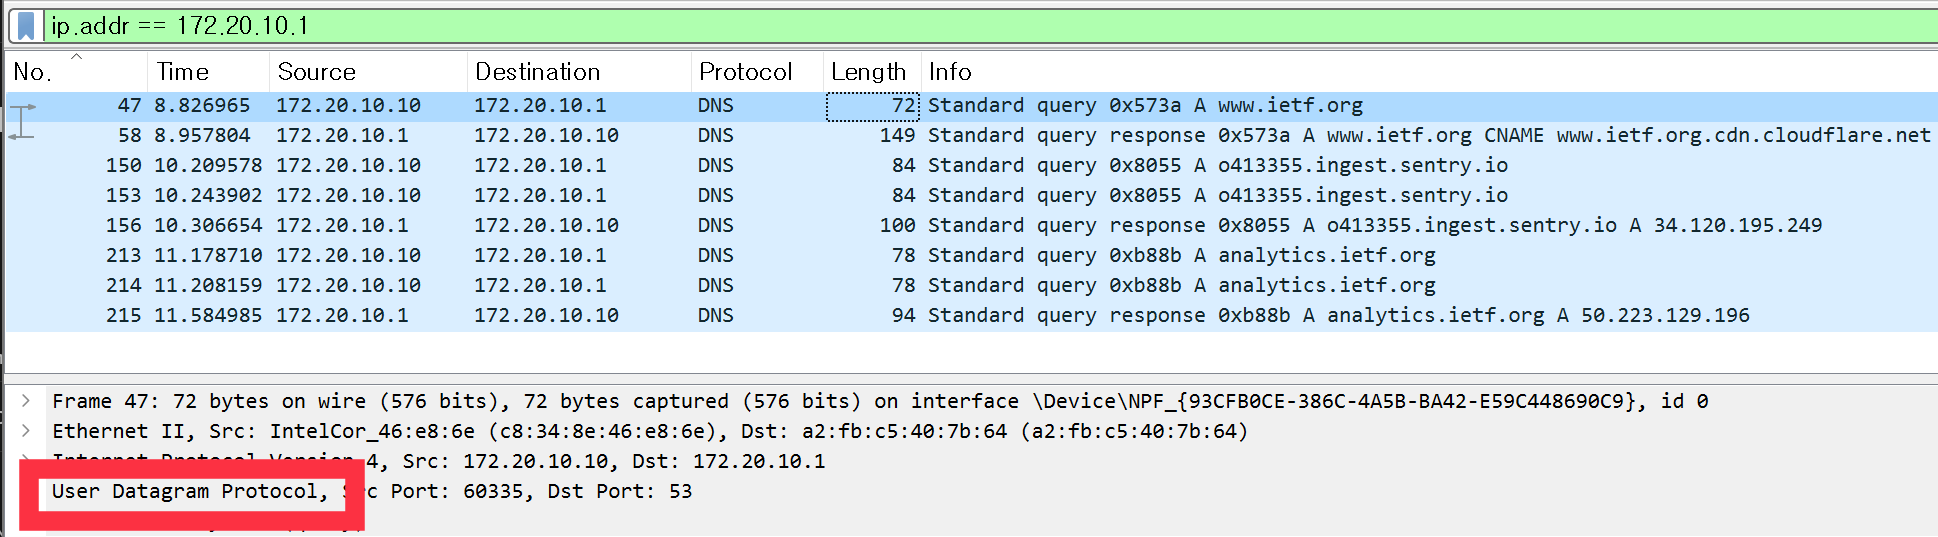
\includegraphics[width=.78\textwidth]{image/result_week01/Q3-1.png}
        		\caption{\footnotesize Problem 3-1's screenshot : DNS over UDP}
        		\vspace{-10pt}
            \end{figure}
            % \vspace{-4mm}
        \item What is the destination port for the DNS query message? 
        What is the source port of DNS response message?\\[0.2mm]
            \soln Both the destination port of the DNS query message and the source port of the DNS response message are port 53.
            \vspace{-2mm}  
            \begin{figure}[!h]\centering
            \hspace{10mm} 
        		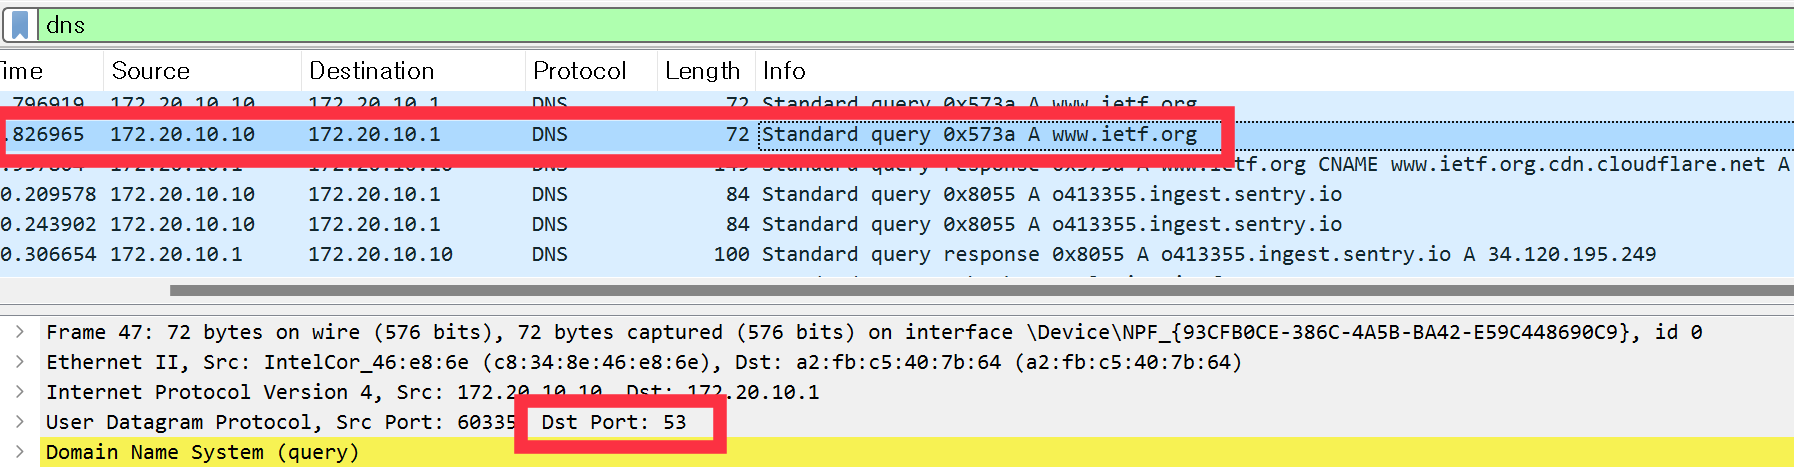
\includegraphics[width=.78\textwidth]{image/result_week01/Q3-2-1.png}
        		\caption{\footnotesize Problem 3-2-1's screenshot : The destination port of the DNS query message}
        		\vspace{-10pt}
            \end{figure}
            % \vspace{-4mm}  
            \begin{figure}[!h]\centering
            \hspace{10mm} 
        		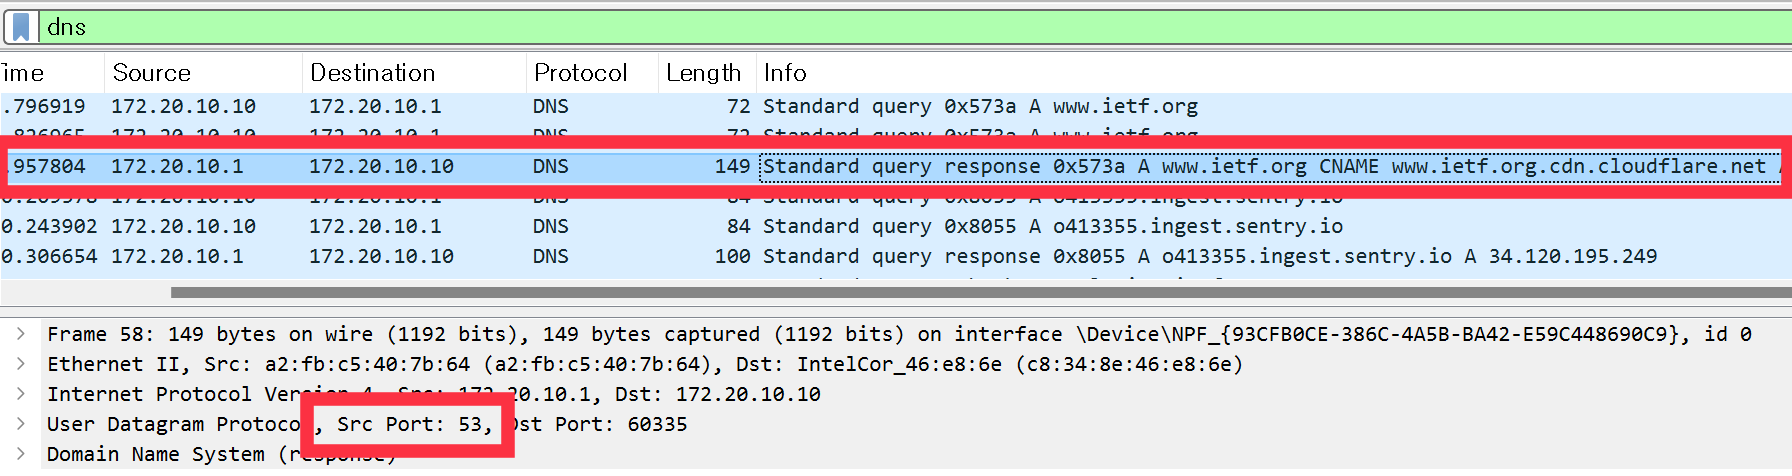
\includegraphics[width=.79\textwidth]{image/result_week01/Q3-2-2.png}
        		\caption{\footnotesize Problem 3-2-2's screenshot : The source port of the DNS reponse message}
        		\vspace{-10pt}
            \end{figure}
        \item To what IP address is the DNS query message sent? 
        Use ipconfig to determine the IP address of your local DNS server. 
        Are these two IP addresses the same?\\[0.2mm]
            \soln The DNS query message sent to IP address ‘172.20.10.1’, which is the same of my local DNS server could be figured out as issued ‘ipconfig /all’ in powershell.
            \vspace{-2mm}
            \begin{figure}[!h]\centering
            \hspace{10mm} 
        		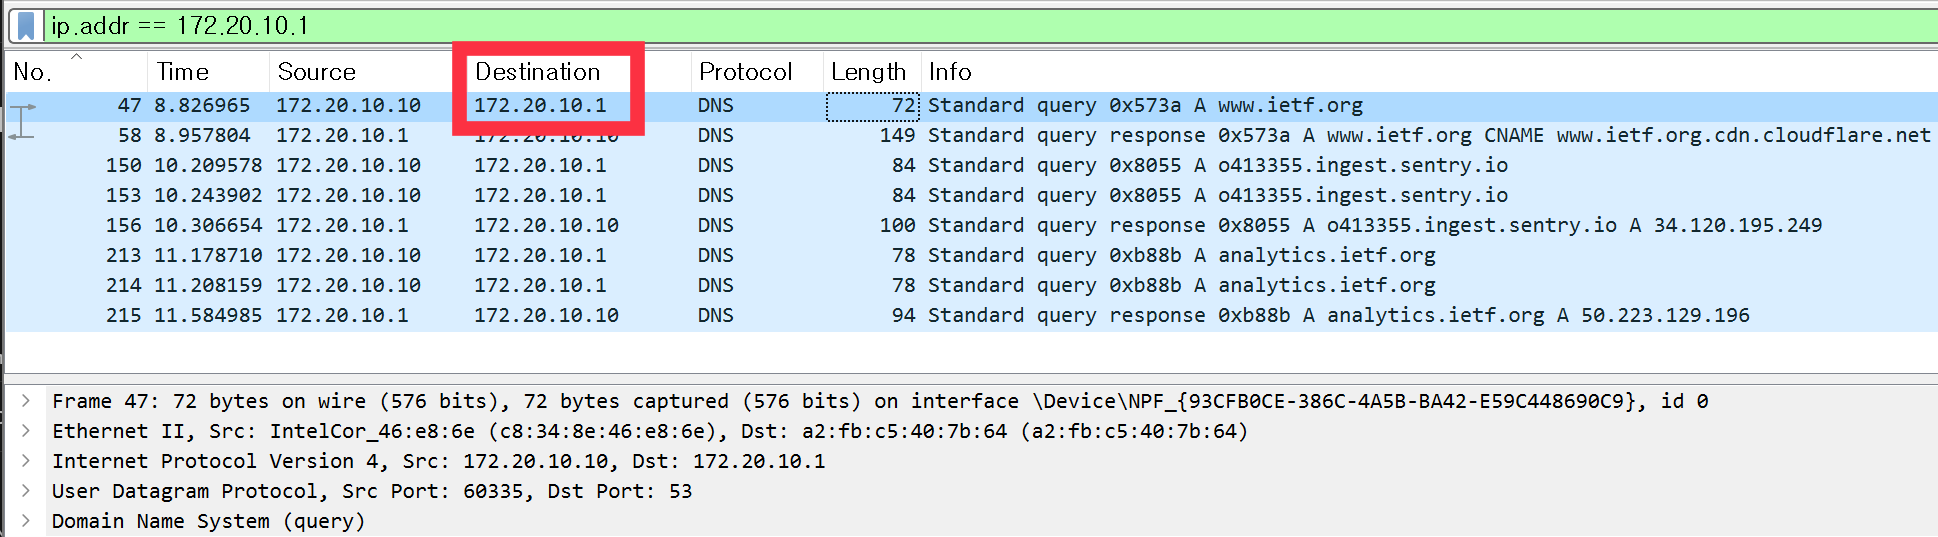
\includegraphics[width=.78\textwidth]{image/result_week01/Q3-3-1.png}
        		\caption{\footnotesize Problem 3-3-1's screenshot : The destination IP adress of DNS query message}
        		\vspace{-10pt}
            \end{figure}
            % \vspace{-4mm}  
            \begin{figure}[!h]\centering
            \hspace{10mm} 
        		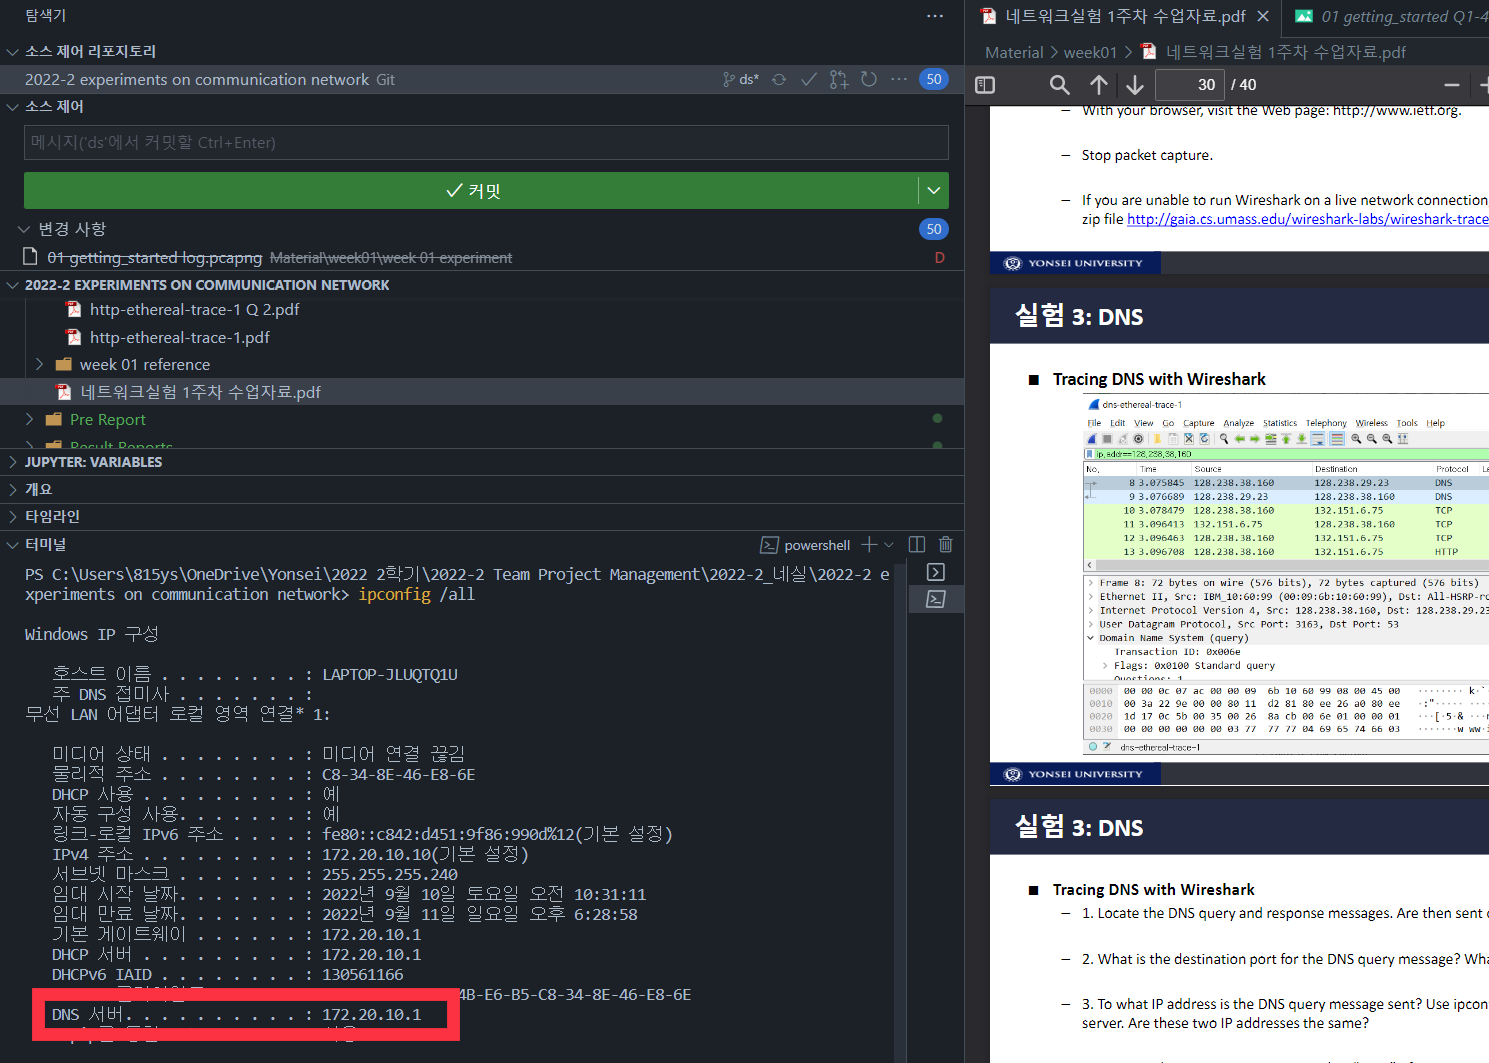
\includegraphics[width=.79\textwidth]{image/result_week01/Q3-3-2.png}
        		\caption{\footnotesize Problem 3-3-2's screenshot : 'ipconfig /all' command in powershell}
        		\vspace{-10pt}
            \end{figure}
        \item Examine the DNS query message. What “Type” of DNS query is it? 
        Does the query message contain any “answers”?\\[0.2mm]
        \soln Type A / The query message doesn’t contain any answers.
            \vspace{-2mm}  
            \begin{figure}[!h]\centering
            \hspace{10mm} 
        		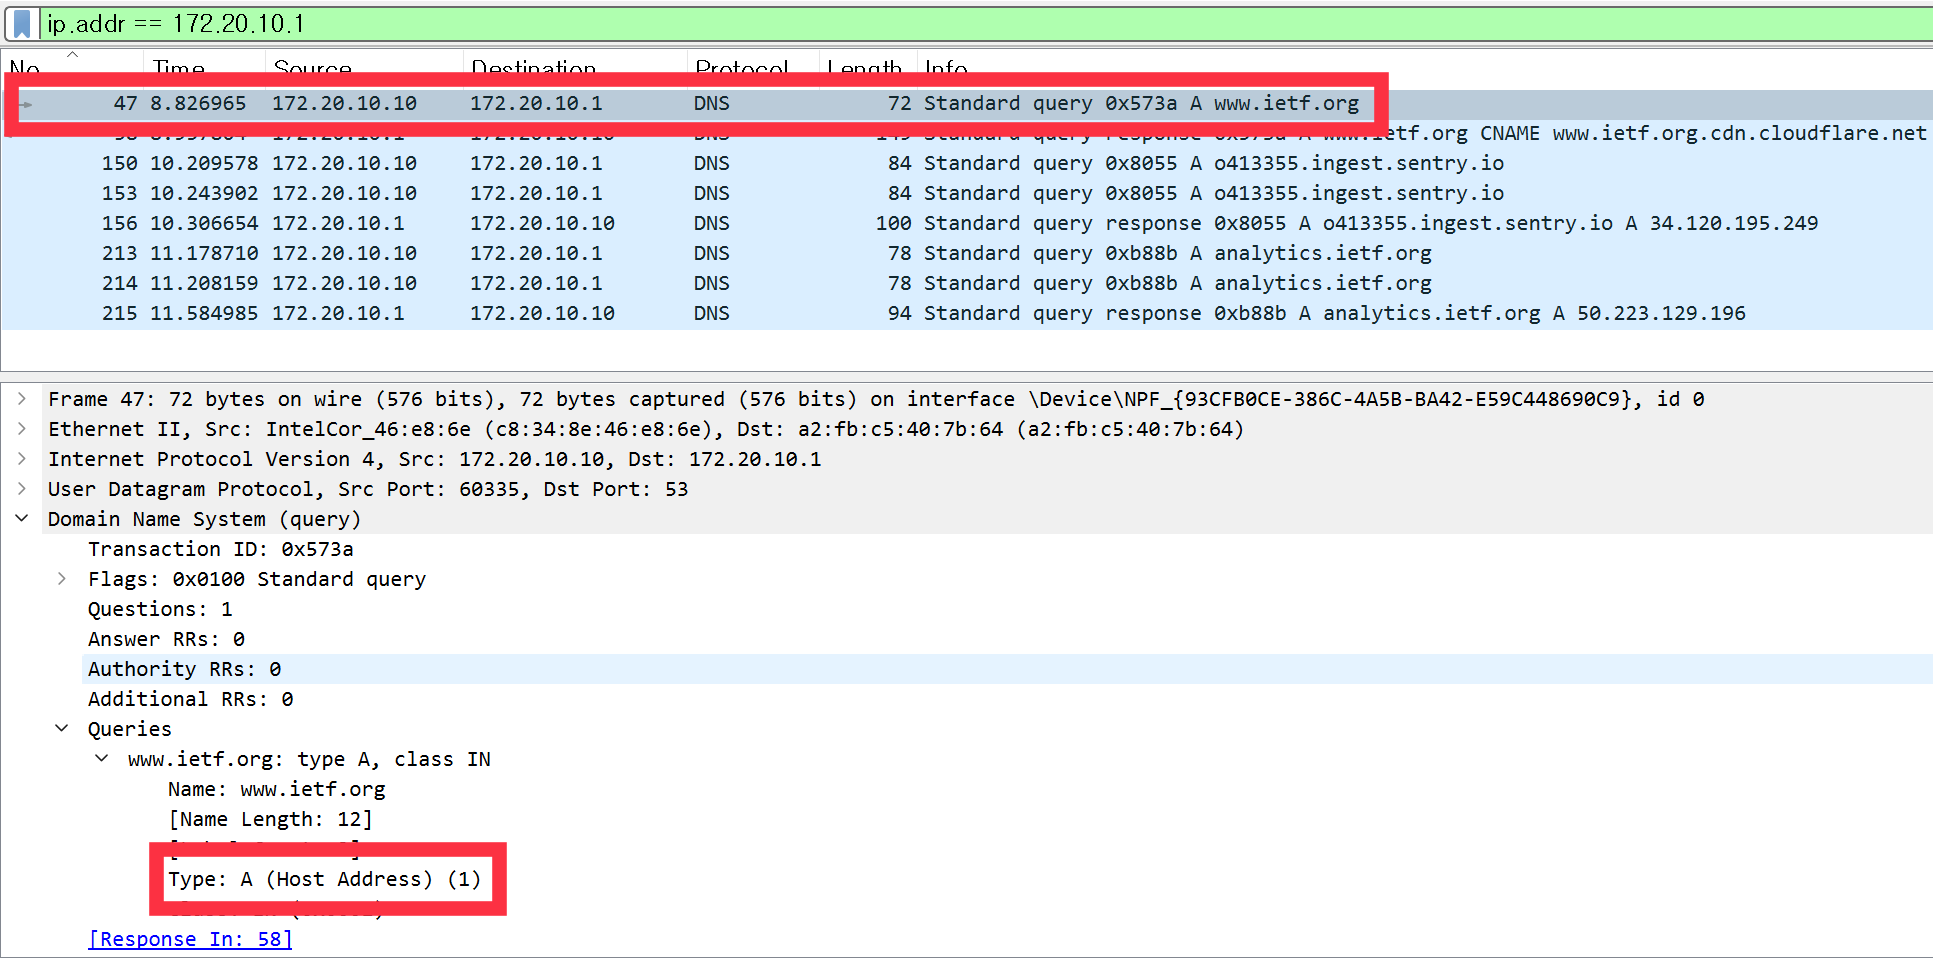
\includegraphics[width=.78\textwidth]{image/result_week01/Q3-4.png}
        		\caption{\footnotesize Problem 3-4's screenshot : DNS query message, Type A}
        		\vspace{-10pt}
            \end{figure}
            % \vspace{-4mm}
\newpage
        \item Examine the DNS response message. How many “answers” are provided? 
        What do each of these answers contain?\\[0.2mm]
            \soln There are three answers which contain information about Name, Type, Class, Time to live, Data length, CNAME.
             \vspace{-2mm}  
            \begin{figure}[!h]\centering
            \hspace{10mm} 
        		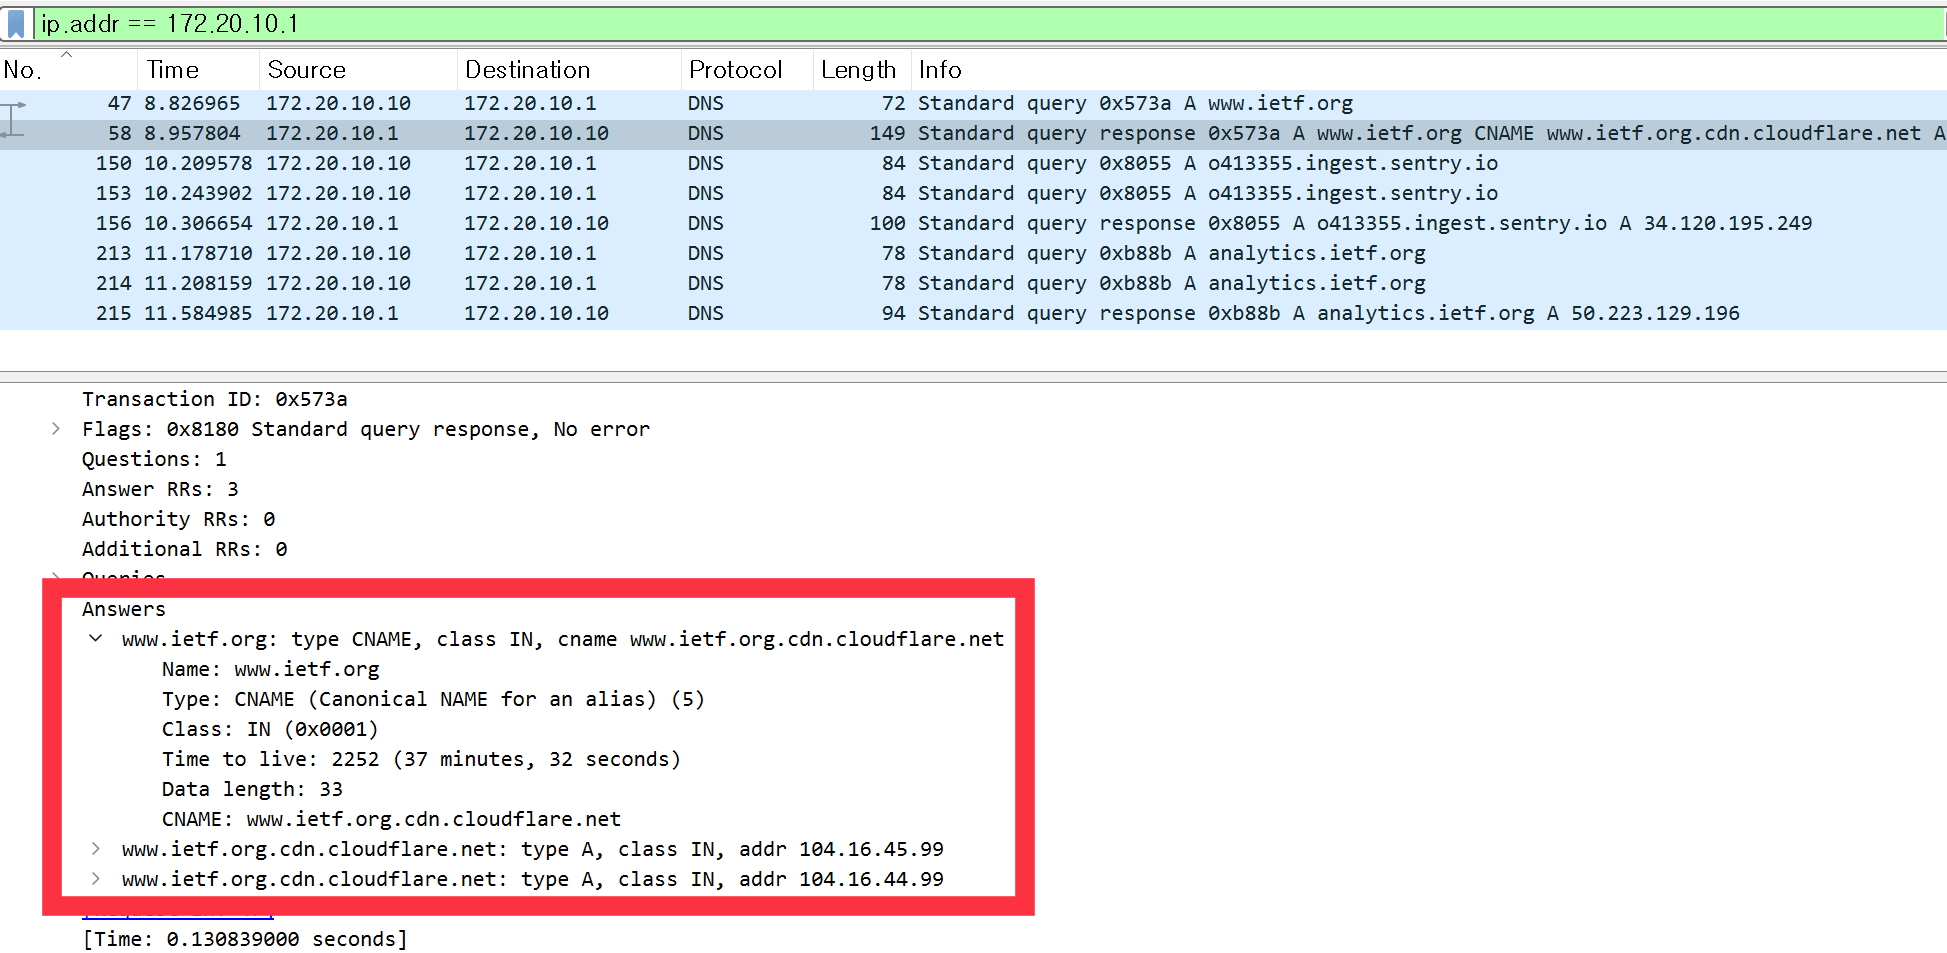
\includegraphics[width=.78\textwidth]{image/result_week01/Q3-5.png}
        		\caption{\footnotesize Problem 3-5's screenshot : DNS query response message, answers}
        		\vspace{-10pt}
            \end{figure}
            % \vspace{-4mm}
        \item Consider the subsequent TCP SYN packet sent by your host.
        Does the destination IP address of the SYN packet correspond to any of the IP addresses 
        provided in the DNS response message?\\[0.2mm]
            \soln The first SYN packet was sent to 104.16.45.99 that corresponds to the IP address provided in the DNS response message.
            \vspace{-2mm}  
            \begin{figure}[!h]\centering
            \hspace{10mm} 
        		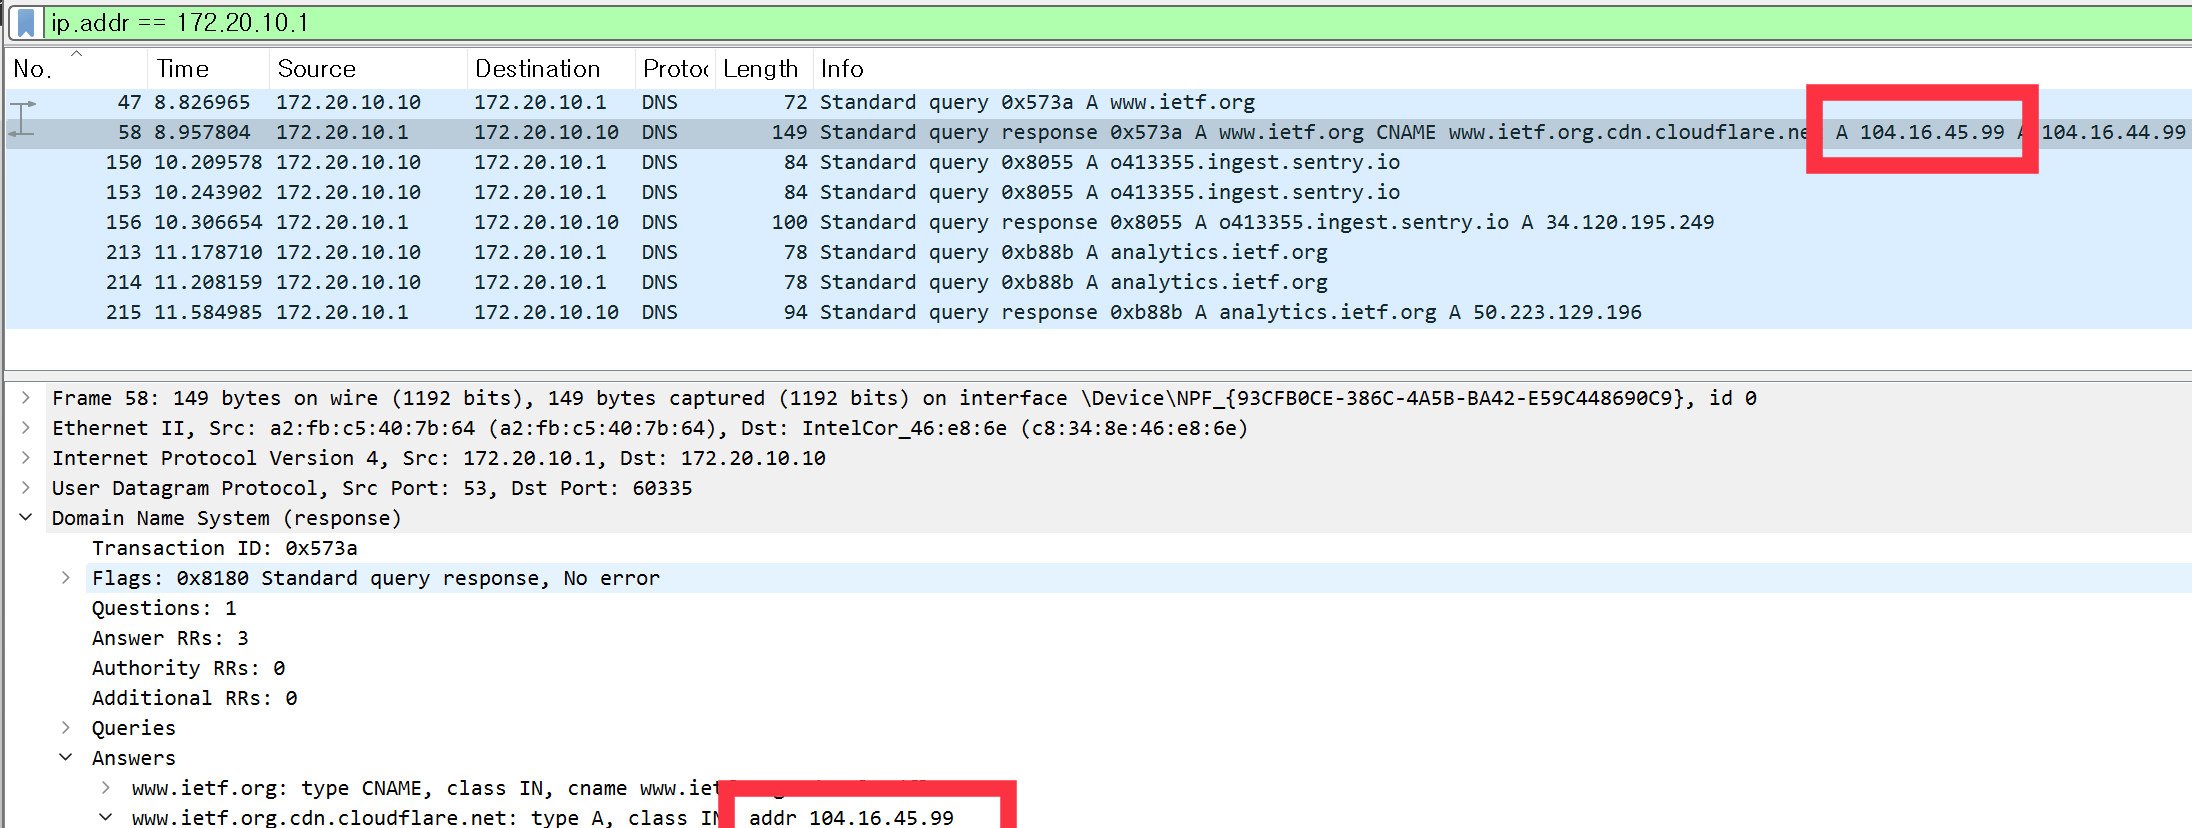
\includegraphics[width=.78\textwidth]{image/result_week01/Q3-6.png}
        		\caption{\footnotesize Problem 3-6's screenshot : IP address provided in DNS query response message}
        		\vspace{-10pt}
            \end{figure}
            % \vspace{-4mm}
        \item This web page contains images. Before retrieving each image, 
        does your host issue new DNS queries?\\[0.2mm]
            \soln There is no any issued DNS queries.
    \end{enumerate}
% Experiment 3-2
\subsection{DNS : Traing DNS with Wireshark \#2}
    \subsubsection*{Experiment Results}
        \vspace{-2mm}  
        \begin{figure}[!h]\centering
            \hspace{10mm} 
    		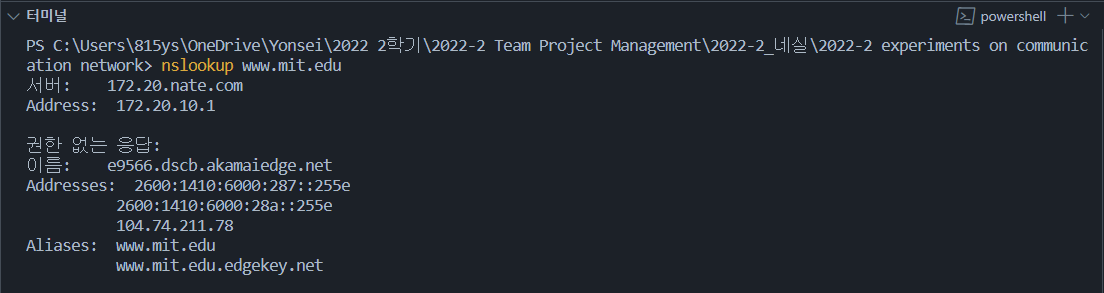
\includegraphics[width=.78\textwidth]{image/result_week01/Q3-8-0.png}
    		\caption{\footnotesize Experiment 3 - b screenshot : 'nslookup' on 'www.mit.edu'}
    		\vspace{-10pt}
        \end{figure}
\clearpage
    \subsubsection*{Problems}
    \begin{enumerate}[label=\bfseries Problem \arabic*:,leftmargin=*,labelindent=1em]\addtocounter{enumi}{7}
        \item What is the destination port for the DNS query message? 
        What is the source port of DNS response message?\\[0.2mm]
            \soln Both the destination port of the DNS query message and the source port of the DNS response message are port 53.

            % \vspace{-4mm}  
            \begin{figure}[!h]\centering
                \hspace{10mm} 
        		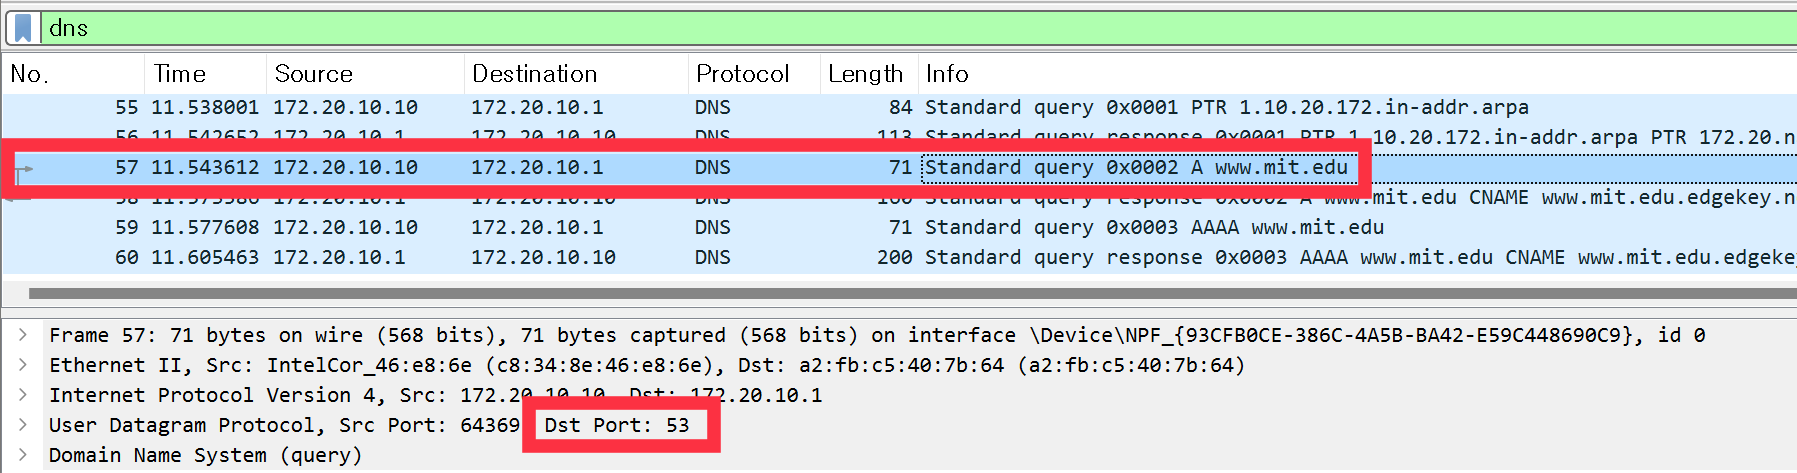
\includegraphics[width=.79\textwidth]{image/result_week01/Q3-8-1.png}
        		\caption{\footnotesize Problem 3-8-1's screenshot : The destination port of the DNS query message}
        		\vspace{-10pt}
            \end{figure}
            % \vspace{-4mm}  
            \begin{figure}[!h]\centering
                \hspace{10mm} 
        		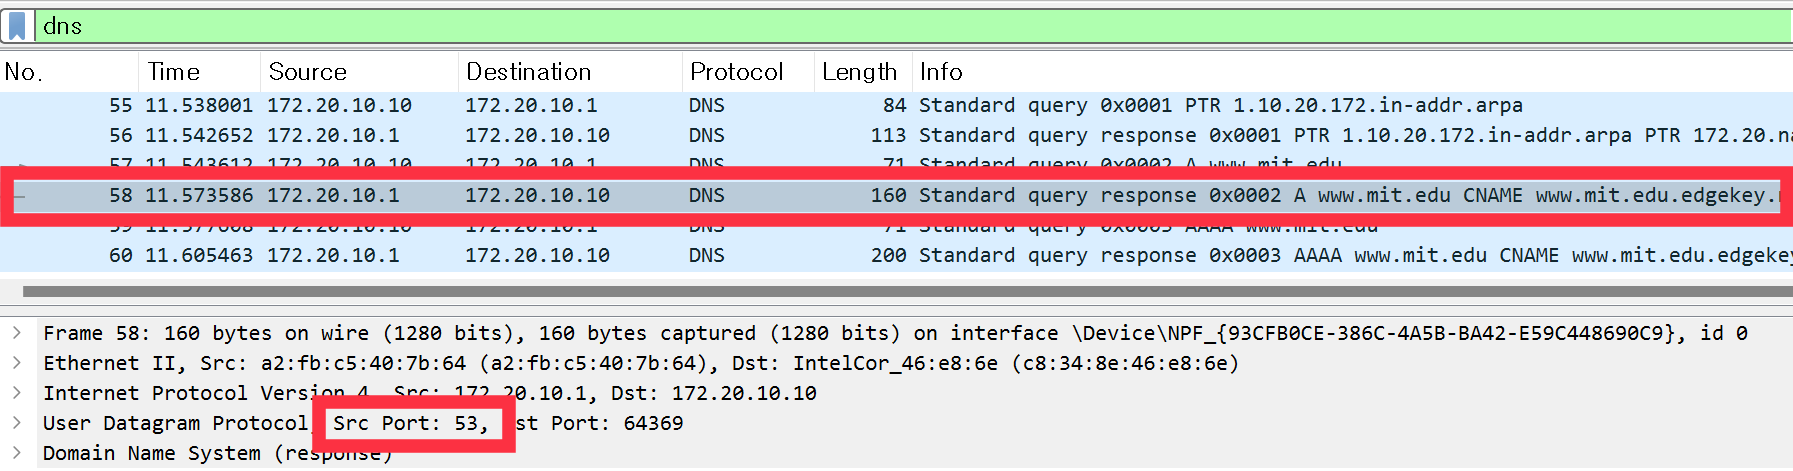
\includegraphics[width=.79\textwidth]{image/result_week01/Q3-8-2.png}
        		\caption{\footnotesize Problem 3-8-2's screenshot : The source port of the DNS response message}
        		\vspace{-10pt}
            \end{figure}
        \item To what IP address is the DNS query message sent? 
        Is this the IP address of your default local DNS server?\\[0.2mm]
            \soln The DNS query message sent to IP addr ‘172.20.10.1’, 
            which is the same of my local DNS server could be figured out as issued ‘ipconfig /all’ in powershell.
            \vspace{-2mm}  
            \begin{figure}[!h]\centering
                \hspace{10mm} 
        		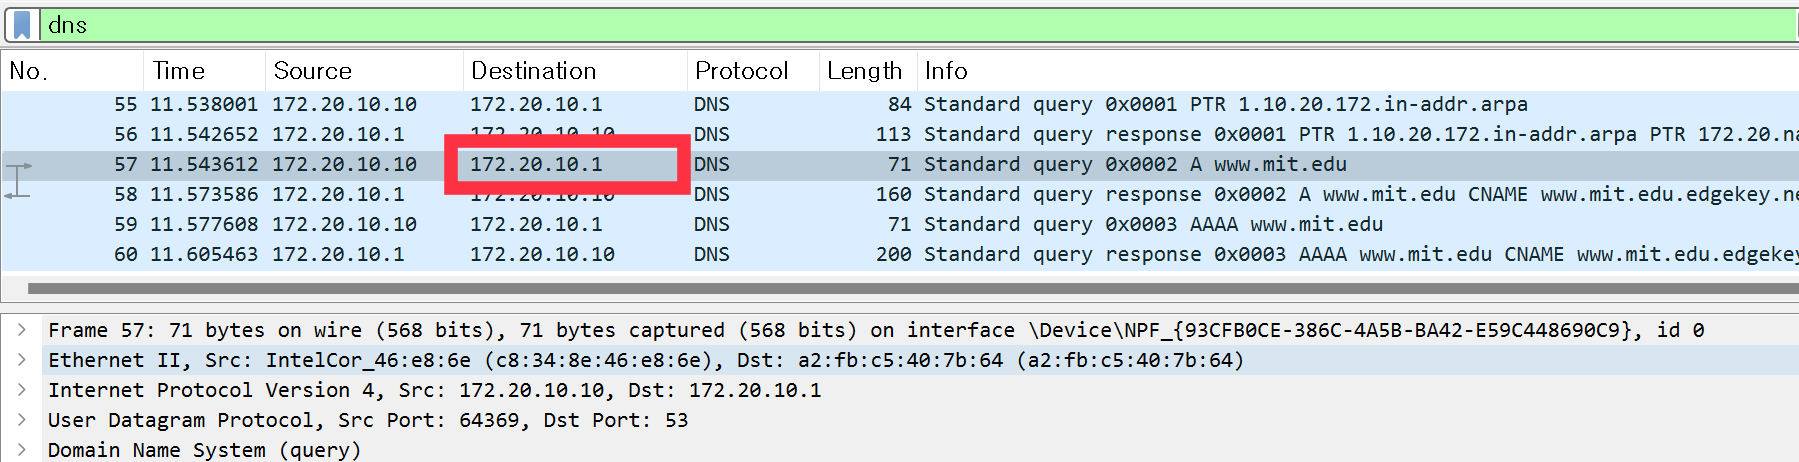
\includegraphics[width=.78\textwidth]{image/result_week01/Q3-9-1.png}
        		\caption{\footnotesize Problem 3-9-1's screenshot : DNS query message}
        		\vspace{-10pt}
            \end{figure}
            % \vspace{-4mm}  
            \begin{figure}[!h]\centering
                \hspace{10mm} 
        		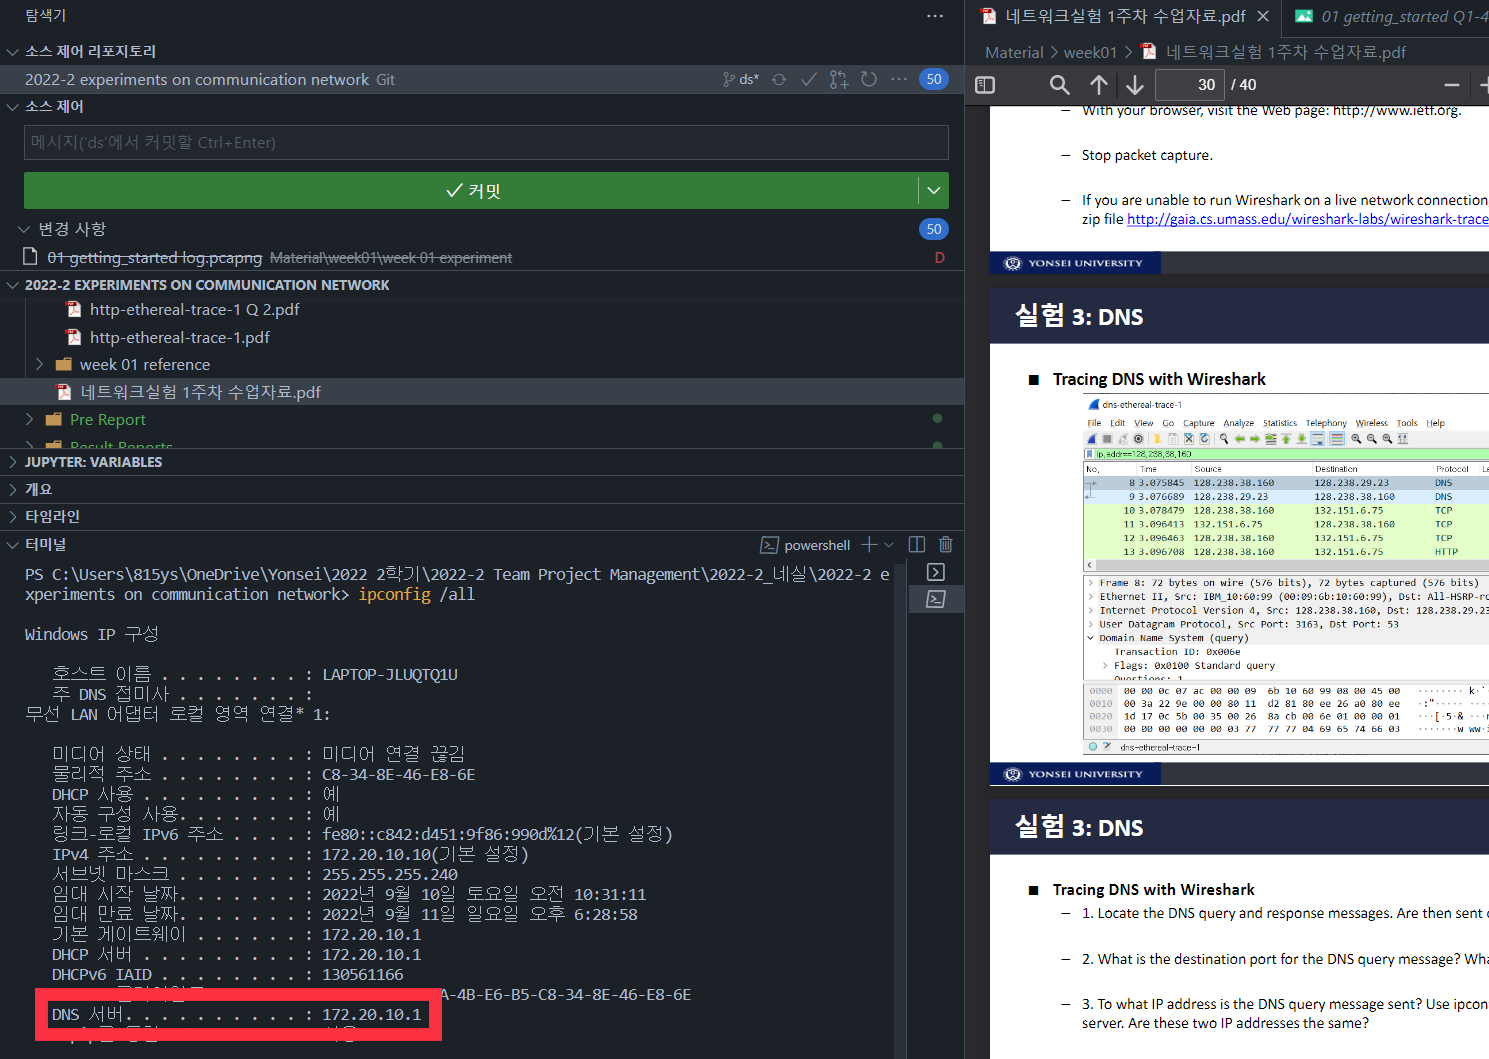
\includegraphics[width=.79\textwidth]{image/result_week01/Q3-9-2.png}
        		\caption{\footnotesize Problem 3-9-2's screenshot : ‘ipconfig /all’ command in powershell}
        		\vspace{-10pt}
            \end{figure}
\clearpage
        \item Examine the DNS query message. What “Type” of DNS query is it? 
        Does the query message contain any “answers”?\\[0.2mm]
            \soln Type A / The query message doesn’t contain any answers.
            \vspace{-2mm}  
            \begin{figure}[!h]\centering
                \hspace{10mm} 
        		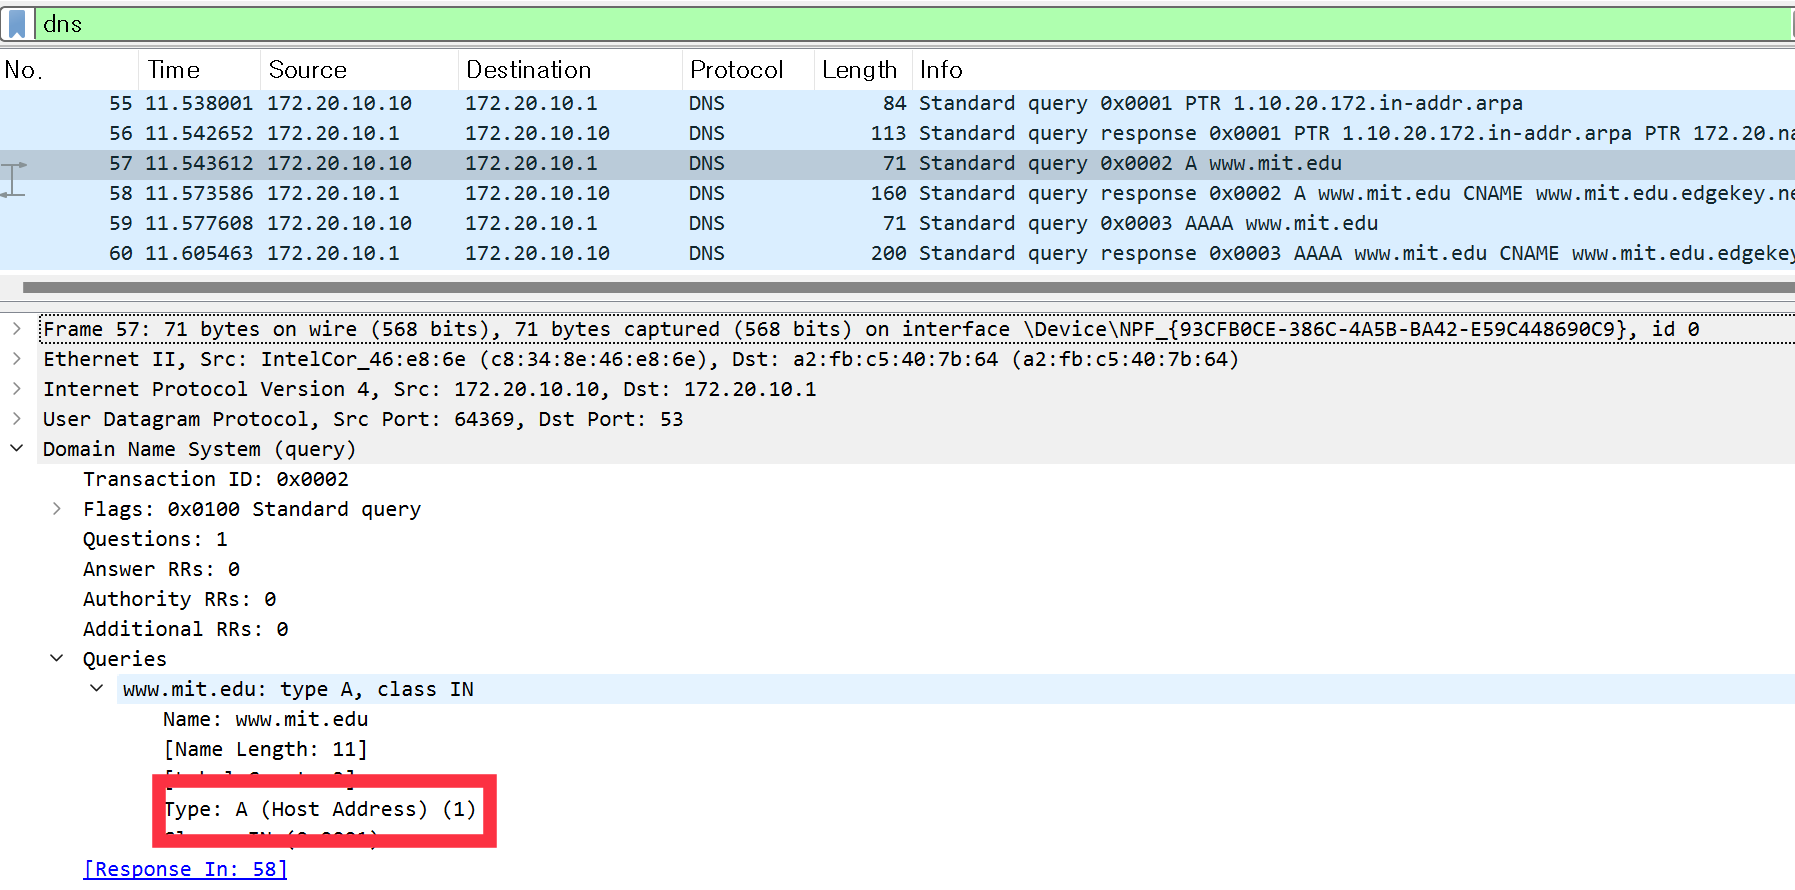
\includegraphics[width=.73\textwidth]{image/result_week01/Q3-a.png}
        		\caption{\footnotesize Problem 3-10's screenshot : DNS query message}
        		\vspace{-10pt}
            \end{figure}
            % \vspace{-4mm}
% \clearpage
        \item Examine the DNS response message. 
        How many “answers” are provided? What do each of these answers contain?\\[0.2mm]
            \soln There are three answers which contains information about Name, Type, Class, Time to live, Data length, CNAME.
            \vspace{-2mm}  
            \begin{figure}[!h]\centering
                \hspace{10mm} 
        		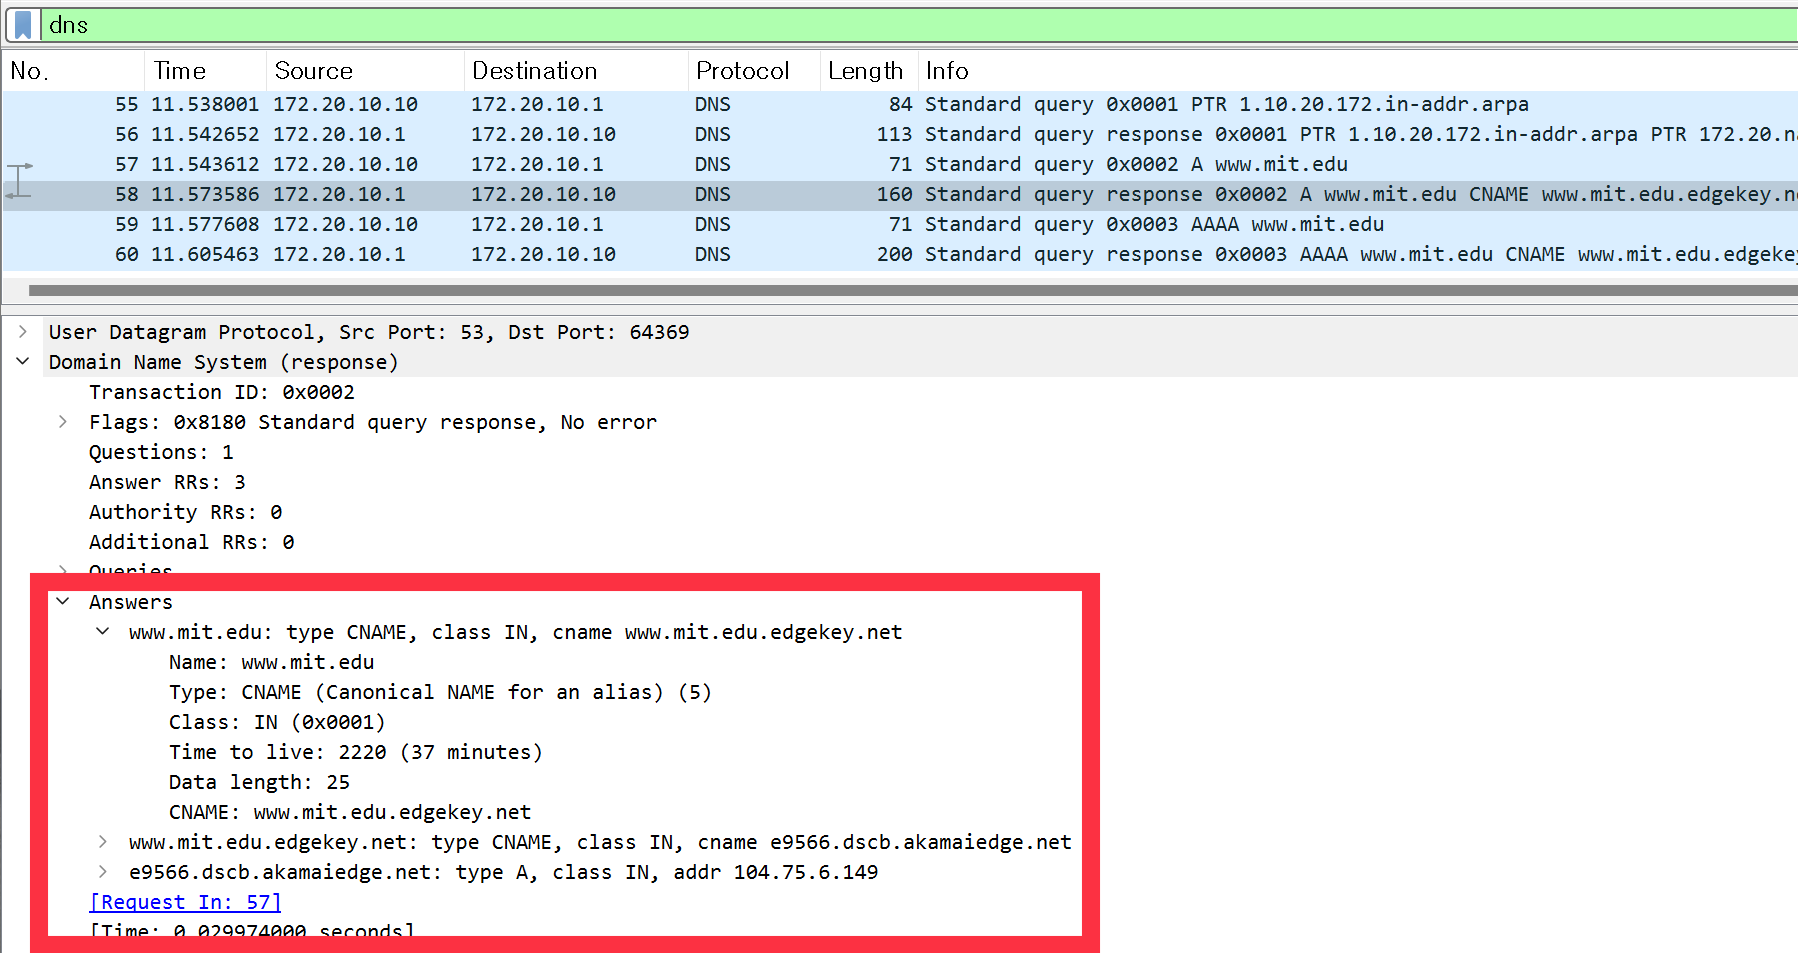
\includegraphics[width=.73\textwidth]{image/result_week01/Q3-b.png}
        		\caption{\footnotesize Problem 3-11's screenshot : DNS response message}
        		\vspace{-10pt}
            \end{figure}
            % \vspace{-4mm}
    \end{enumerate}
% Experiment 3-3
\subsection{DNS : Traing DNS with Wireshark \#3}
    \subsubsection*{Experiment Results}
        \vspace{-2mm}  
        \begin{figure}[!h]\centering
            \hspace{10mm} 
    		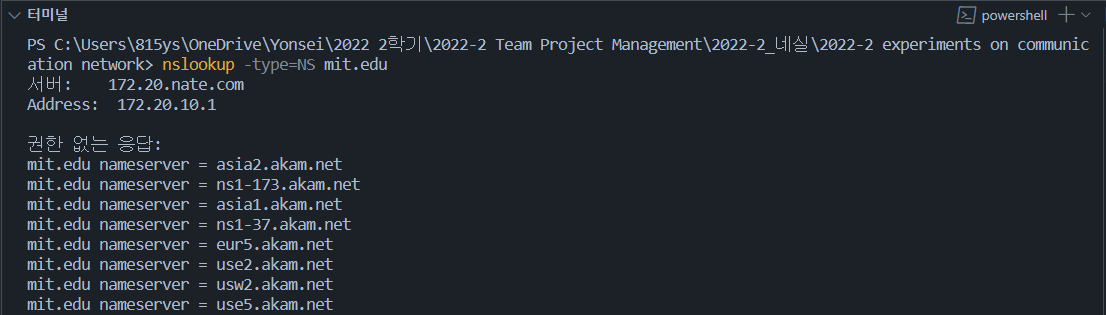
\includegraphics[width=.78\textwidth]{image/result_week01/Q3-c-0.png}
    		\caption{\footnotesize Experiment 3 - C screenshot : 'nslookup -type=NS mit.edu' command in powershell}
    		\vspace{-10pt}
        \end{figure}
\clearpage
    \subsubsection*{Problems}
    \begin{enumerate}[label=\bfseries Problem \arabic*:,leftmargin=*,labelindent=1em]\addtocounter{enumi}{11}
        \item To what IP address is the DNS query message sent? 
        Is this the IP address of your default local DNS server?\\[0.2mm]
            \soln The DNS query message sent to IP addr ‘172.20.10.1’,
            which is the same of my local DNS server could be figured out as issued ‘ipconfig /all’ in powershell.
            % \vspace{-4mm}  
            \begin{figure}[!h]\centering
                \hspace{10mm} 
        		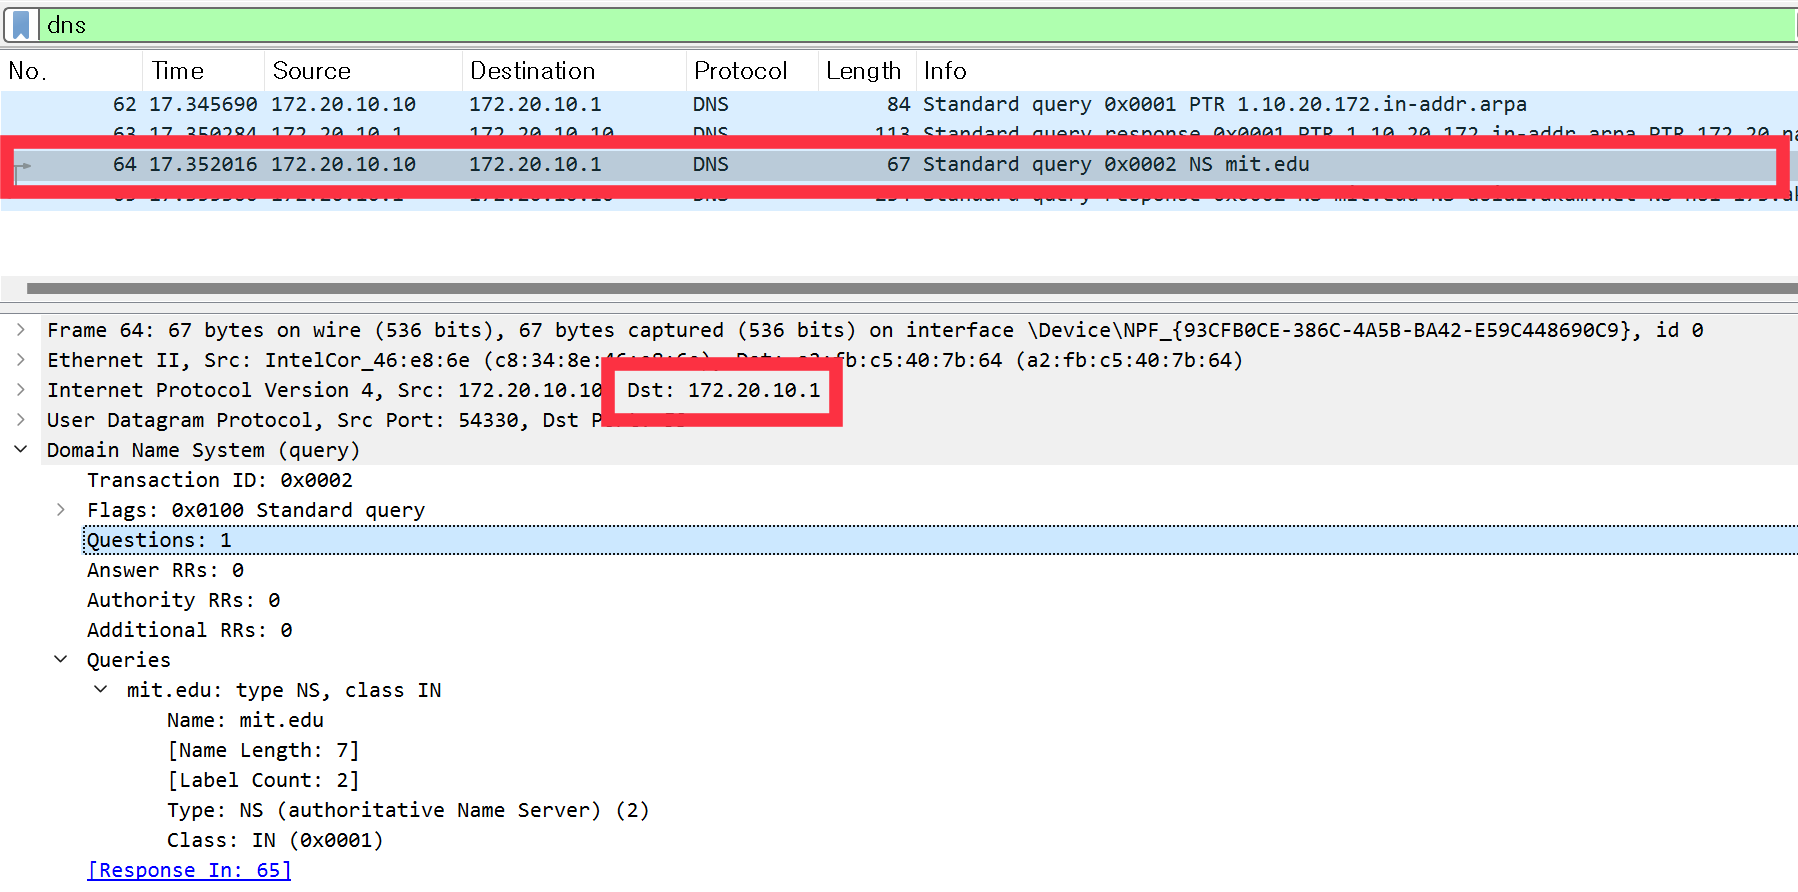
\includegraphics[width=.79\textwidth]{image/result_week01/Q3-c-1.png}
        		\caption{\footnotesize Problem 3-12-1's screenshot : DNS query message}
        		\vspace{-10pt}
            \end{figure}
            % \vspace{-4mm}  
            \begin{figure}[!h]\centering
                \hspace{10mm} 
        		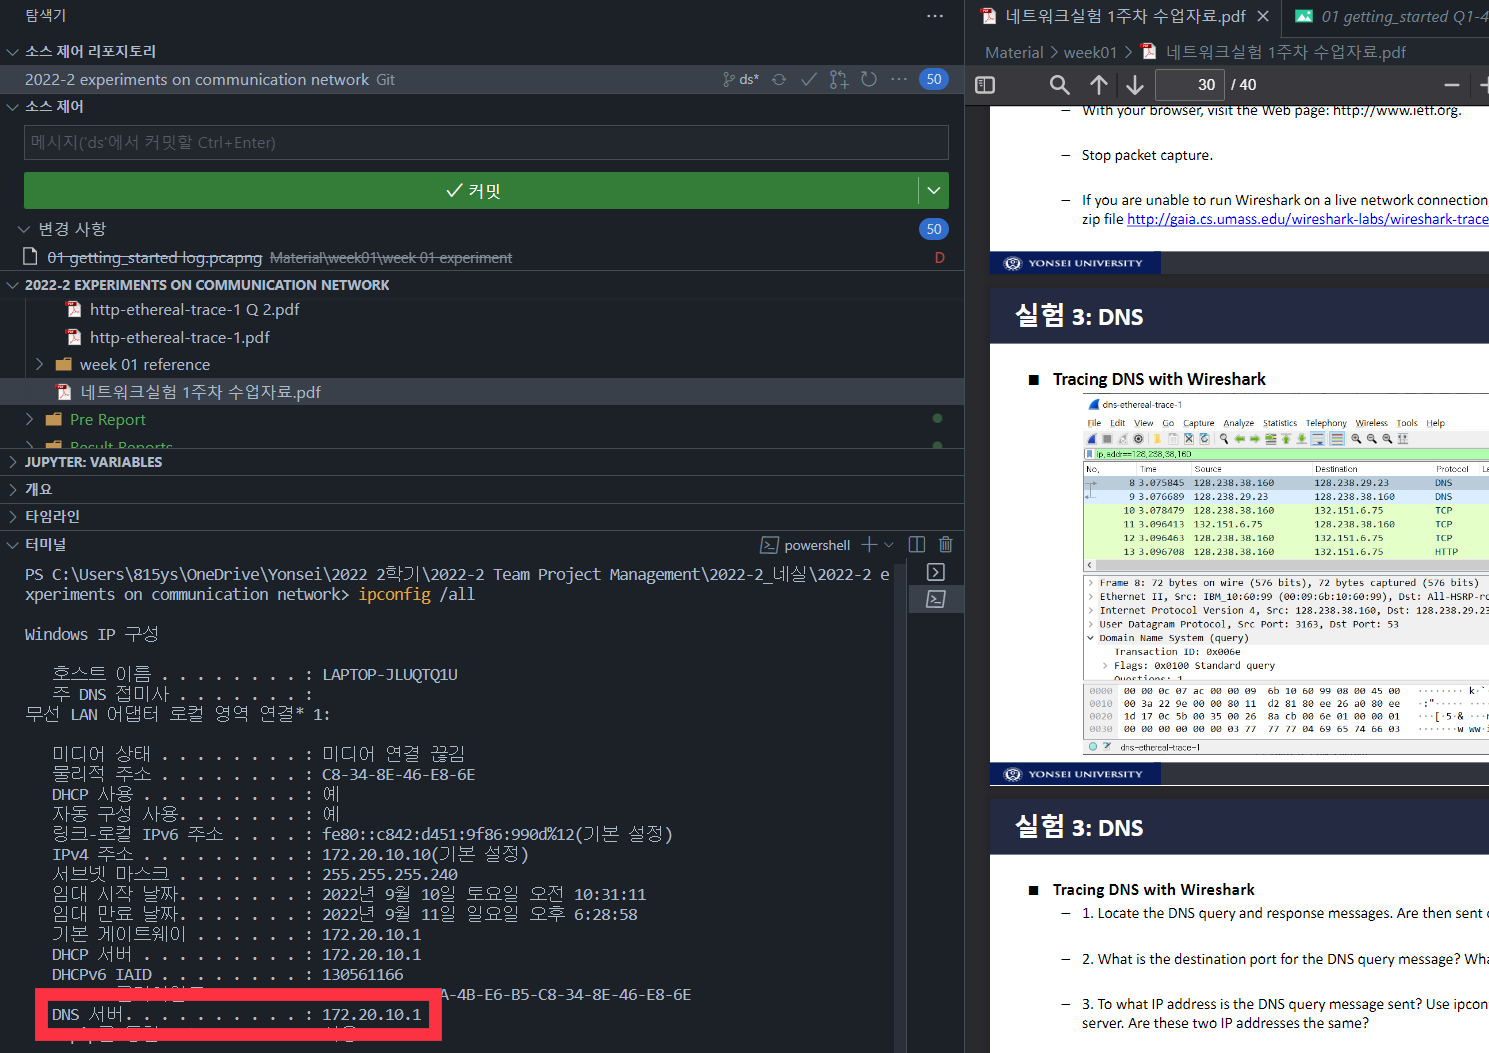
\includegraphics[width=.79\textwidth]{image/result_week01/Q3-c-2.png}
        		\caption{\footnotesize Problem 3-12-2's screenshot : Local DNS server}
        		\vspace{-10pt}
            \end{figure}
        \item Examine the DNS query message. What “Type” of DNS query is it? 
        Does the query message contain any “answers”?\\[0.2mm]
            \soln Type NS\footnote{Name Server} / The query message doesn’t contain any answers.
            \vspace{-2mm}  
            \begin{figure}[!h]\centering
                \hspace{10mm} 
        		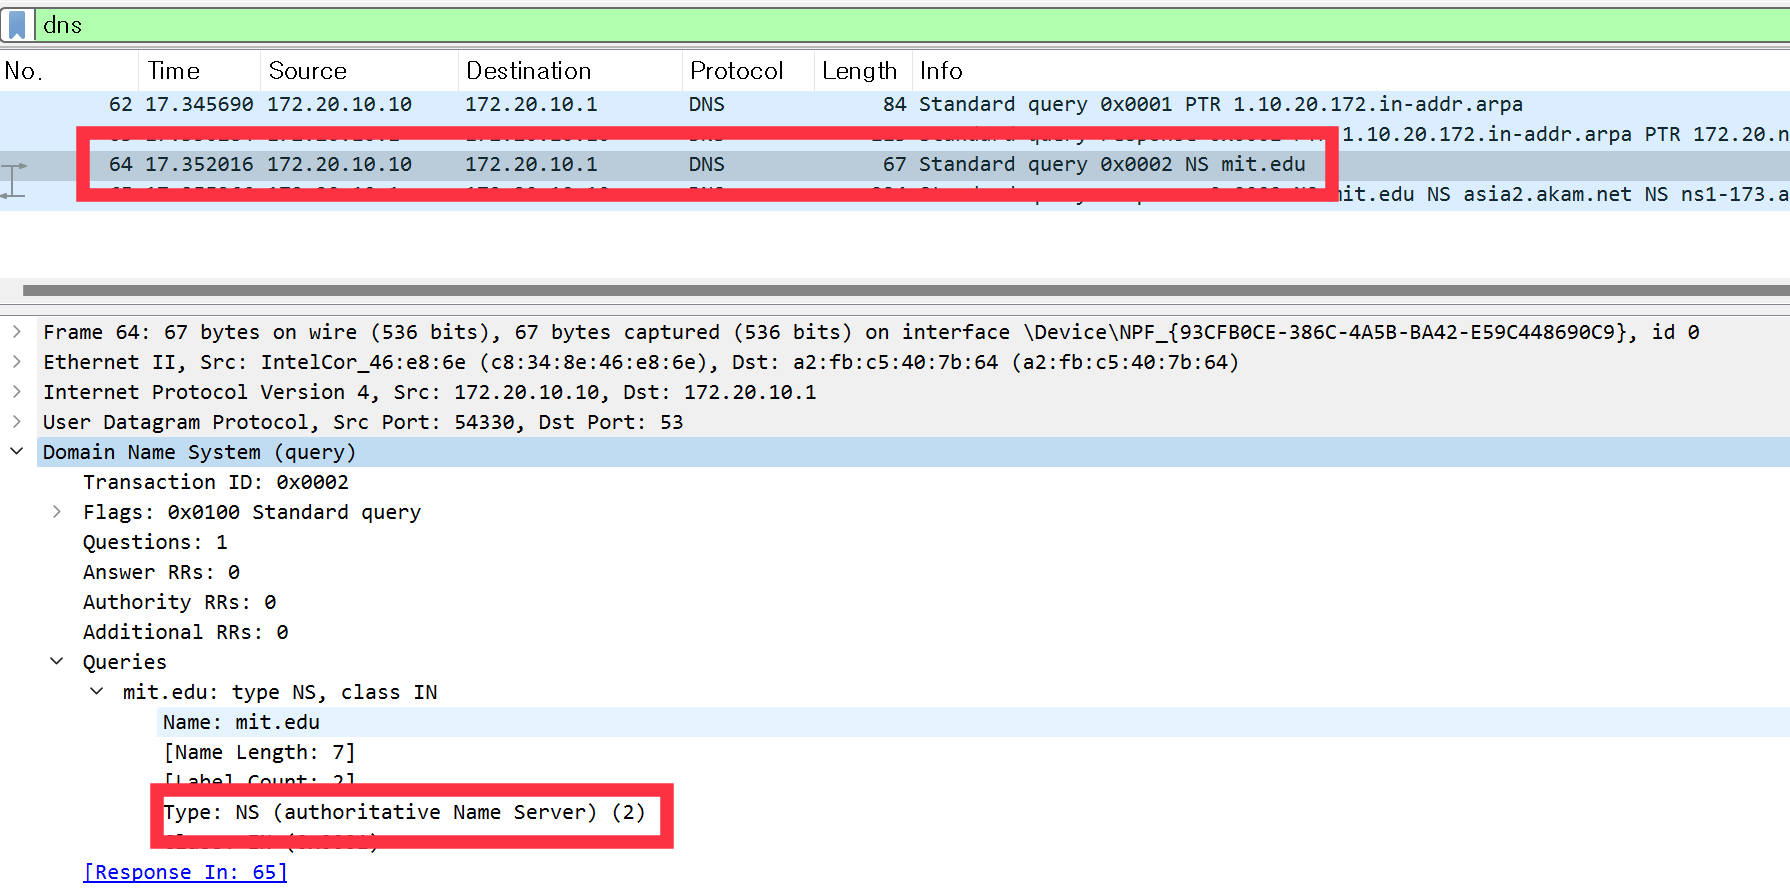
\includegraphics[width=.78\textwidth]{image/result_week01/Q3-d.png}
        		\caption{\footnotesize Problem 3-13's screenshot : DNS query message}
        		\vspace{-10pt}
            \end{figure}
            % \vspace{-4mm}
        \item Examine the DNS response message. What MIT nameservers does the response message provide? 
        Does this response message also provide the IP addresses of the MIT nameservers?\\[0.2mm]
            \soln The response message from MIT nameservers provides the information of NAME, TYPE, CLASS, TIME TO LIVE, DATA LENGTH and NAME SERVER.\\ 
            No. They provided the name of the nameserver such as ‘asia1.akam.net’, ‘ns1-37.akam.net’, but they don’t provide the IP address of the nameserver.
            \vspace{-2mm}  
            \begin{figure}[!h]\centering
                \hspace{10mm} 
        		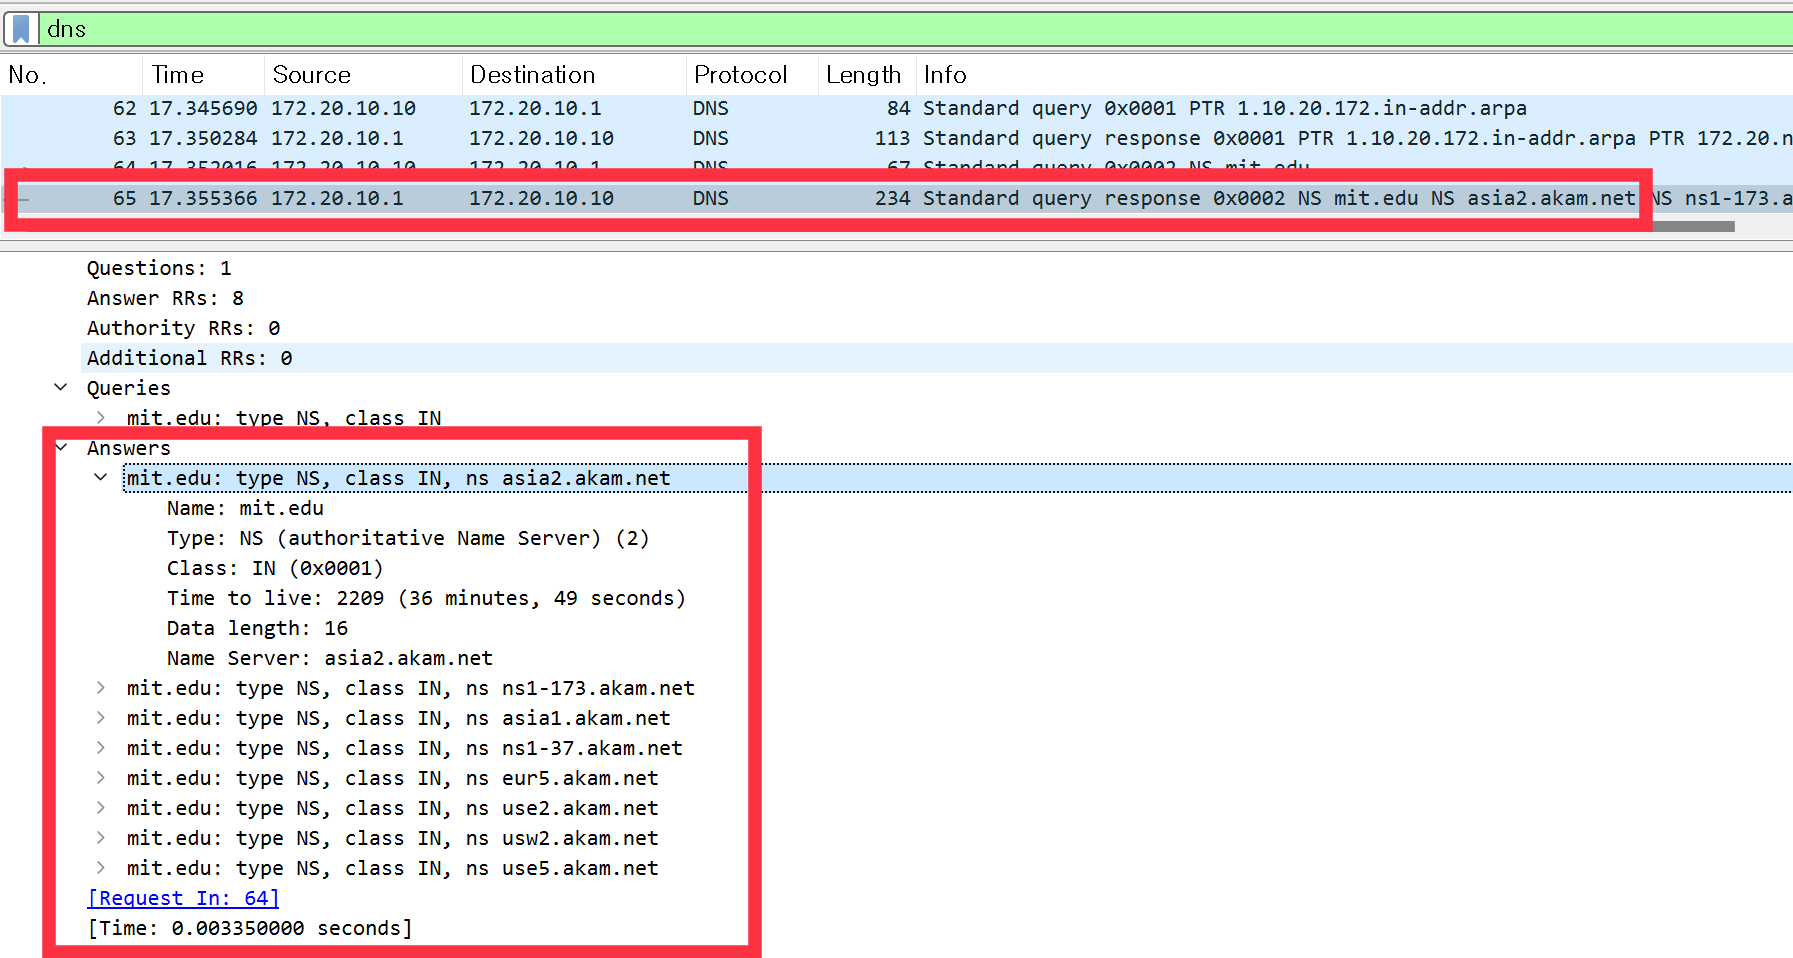
\includegraphics[width=.78\textwidth]{image/result_week01/Q3-e-1.png}
        		\caption{\footnotesize Problem 3-14-1's screenshot : DNS query response message}
        		\vspace{-10pt}
            \end{figure}
            % \vspace{-4mm}  
            \begin{figure}[!h]\centering
                \hspace{10mm} 
        		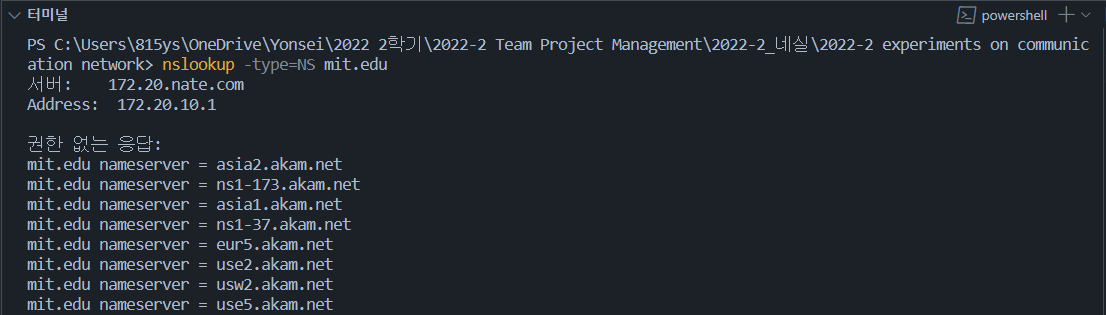
\includegraphics[width=.79\textwidth]{image/result_week01/Q3-e-2.png}
        		\caption{\footnotesize Problem 3-14-2's screenshot : 'nslookup -type=NS mit.edu' command in powershell}
        		\vspace{-10pt}
            \end{figure}
    \end{enumerate}
% Experiment 3-4
\subsection{DNS : Traing DNS with Wireshark \#4}
    \subsubsection*{Experiment Results}
         \vspace{-2mm}  
        \begin{figure}[!h]\centering
            \hspace{10mm} 
    		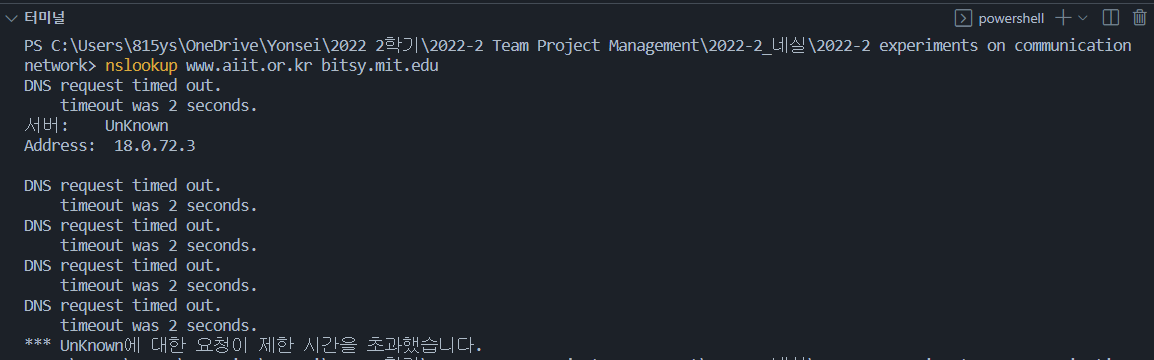
\includegraphics[width=.78\textwidth]{image/result_week01/Q3-f-0.png}
    		\caption{\footnotesize Experiment 3 - d screenshot : 'nslookup www.aiit.co.kr bitsy.mit.edu' command in powershell}
    		\vspace{-10pt}
        \end{figure}
    \subsubsection*{Problems}
    \begin{enumerate}[label=\bfseries Problem \arabic*:,leftmargin=*,labelindent=1em]\addtocounter{enumi}{14}
        \item To what IP address is the DNS query message sent? 
        Is this the IP address of your default local DNS server? 
        If not, what does the IP address correspond to?\\[0.2mm]
            \soln No. DNS query message sent to ‘18.0.72.3’ which is the bitsy.mit.edu’s IP address. 
            And we can figure out this in query response message’s answer from bitsy.mit.edu.

            % \vspace{-4mm}  
            \begin{figure}[!h]\centering
                \hspace{10mm} 
        		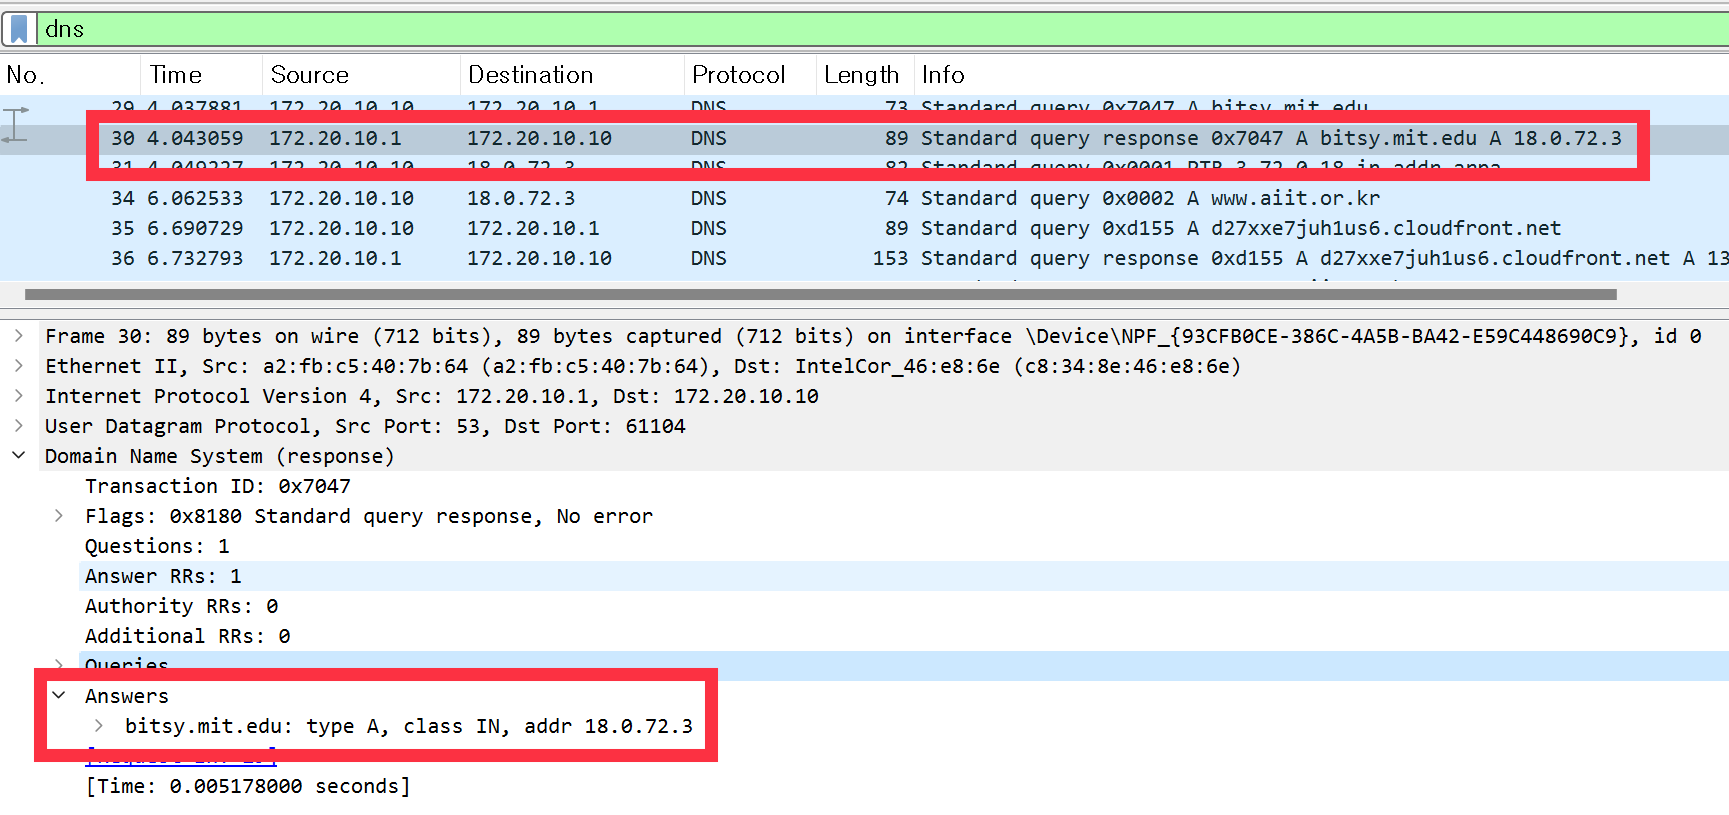
\includegraphics[width=.79\textwidth]{image/result_week01/Q3-f-1.png}
        		\caption{\footnotesize Problem 3-15-1's screenshot : DNS query message}
        		\vspace{-10pt}
            \end{figure}
            % \vspace{-4mm}  
            \begin{figure}[!h]\centering
                \hspace{10mm} 
        		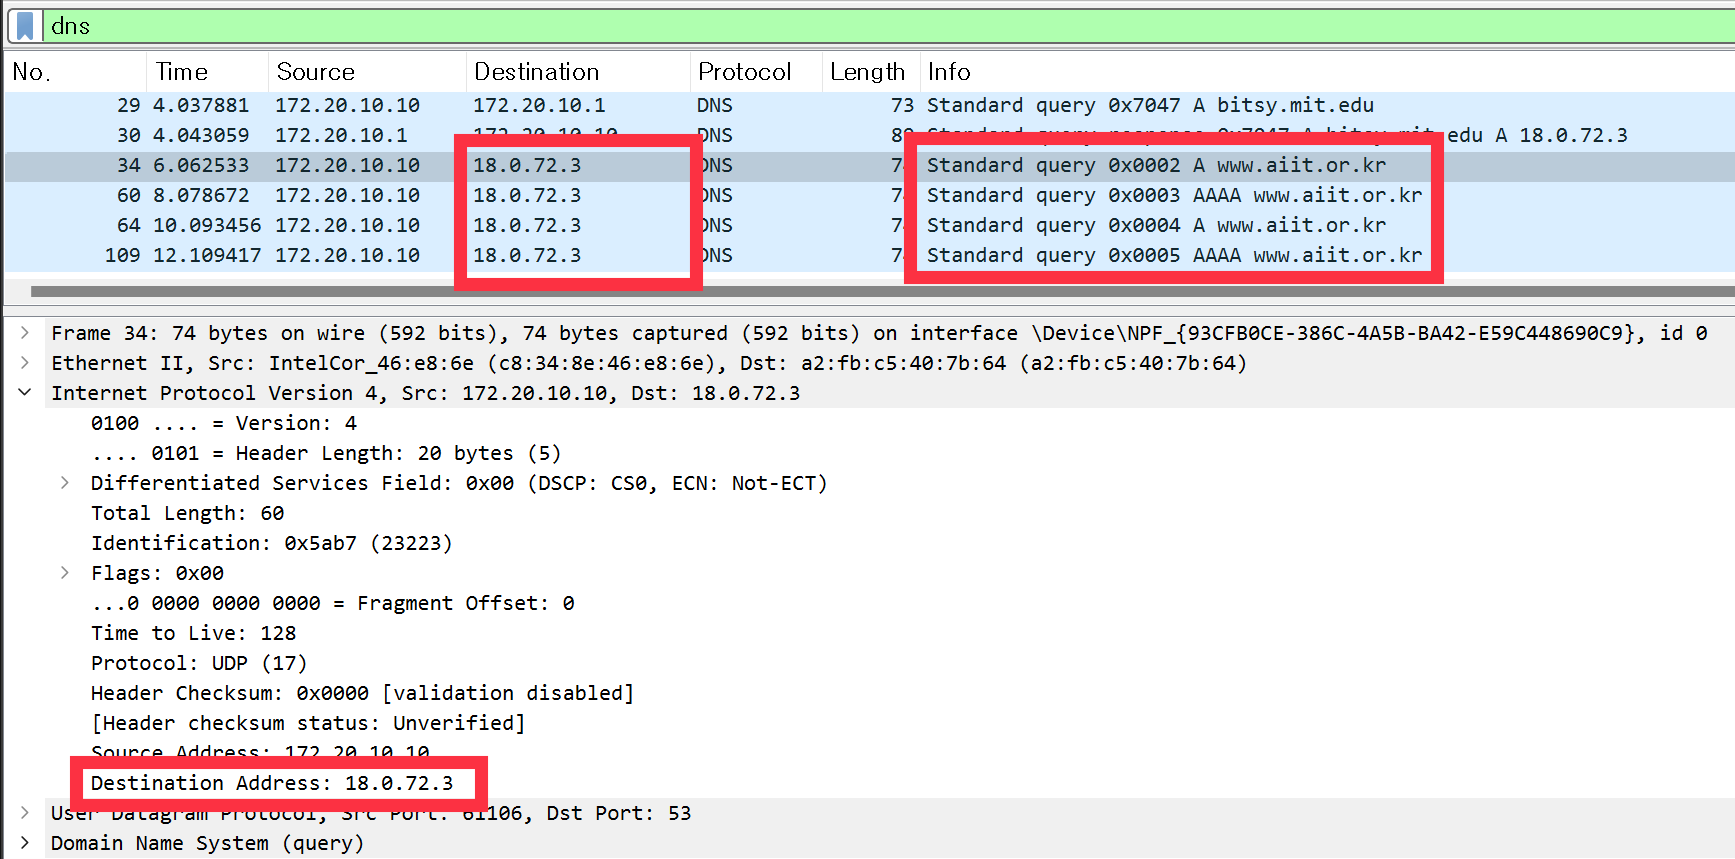
\includegraphics[width=.79\textwidth]{image/result_week01/Q3-f-2.png}
        		\caption{\footnotesize Problem 3-15-2's screenshot : DNS query response message, answers}
        		\vspace{-10pt}
            \end{figure}
        \item Examine the DNS query message. 
        What “Type” of DNS query is it? Does the query message contain any “answers”?\\[0.2mm]
            \soln Type A / The query message doesn’t contain any answers.
            \vspace{-2mm}  
            \begin{figure}[!h]\centering
                \hspace{10mm} 
        		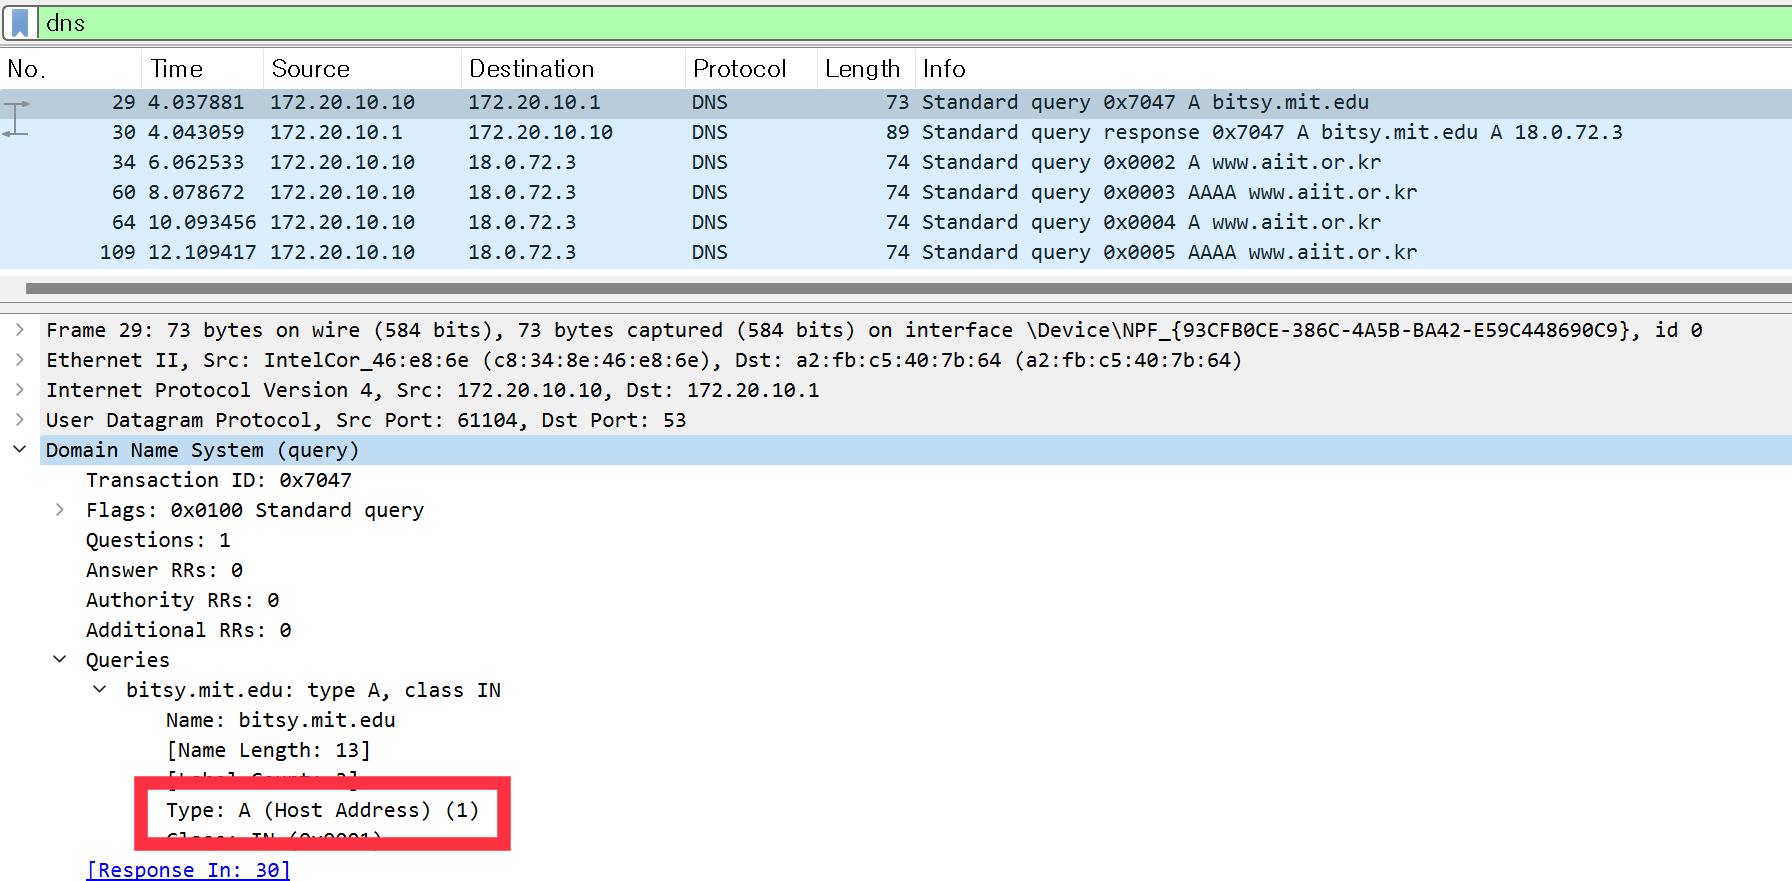
\includegraphics[width=.78\textwidth]{image/result_week01/Q3-g.png}
        		\caption{\footnotesize Problem 3-16's screenshot : DNS query message}
        		\vspace{-10pt}
            \end{figure}
            % \vspace{-4mm}
        \item Examine the DNS response message. How many “answers” are provided?
        What does each of these answers contain?\\[0.2mm]
            \soln As we can see in the figure below, the response from 18.0.72.3 was not received in the DNS request in this experiment.Therefore,
            the answer for question 17 is to use the ‘dns-etheral-trace-4’ file.\\
            One answer was provided. And the answer contained NAME, TYPE, CLASS, TIME TO LIVE, DATA LENGTH and ADDRESS.
            \vspace{-2mm}  
            \begin{figure}[!h]\centering
                \hspace{10mm} 
        		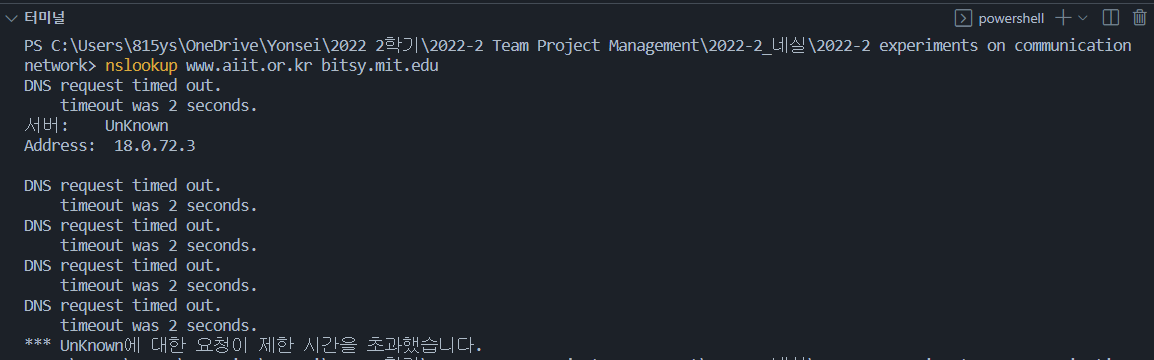
\includegraphics[width=.78\textwidth]{image/result_week01/Q3-h-1.png}
        		\caption{\footnotesize Problem 3-17-1's screenshot : 'nslookup' command in powershell}
        		\vspace{-10pt}
            \end{figure}
            % \vspace{-4mm}  
            \begin{figure}[!h]\centering
                \hspace{10mm} 
        		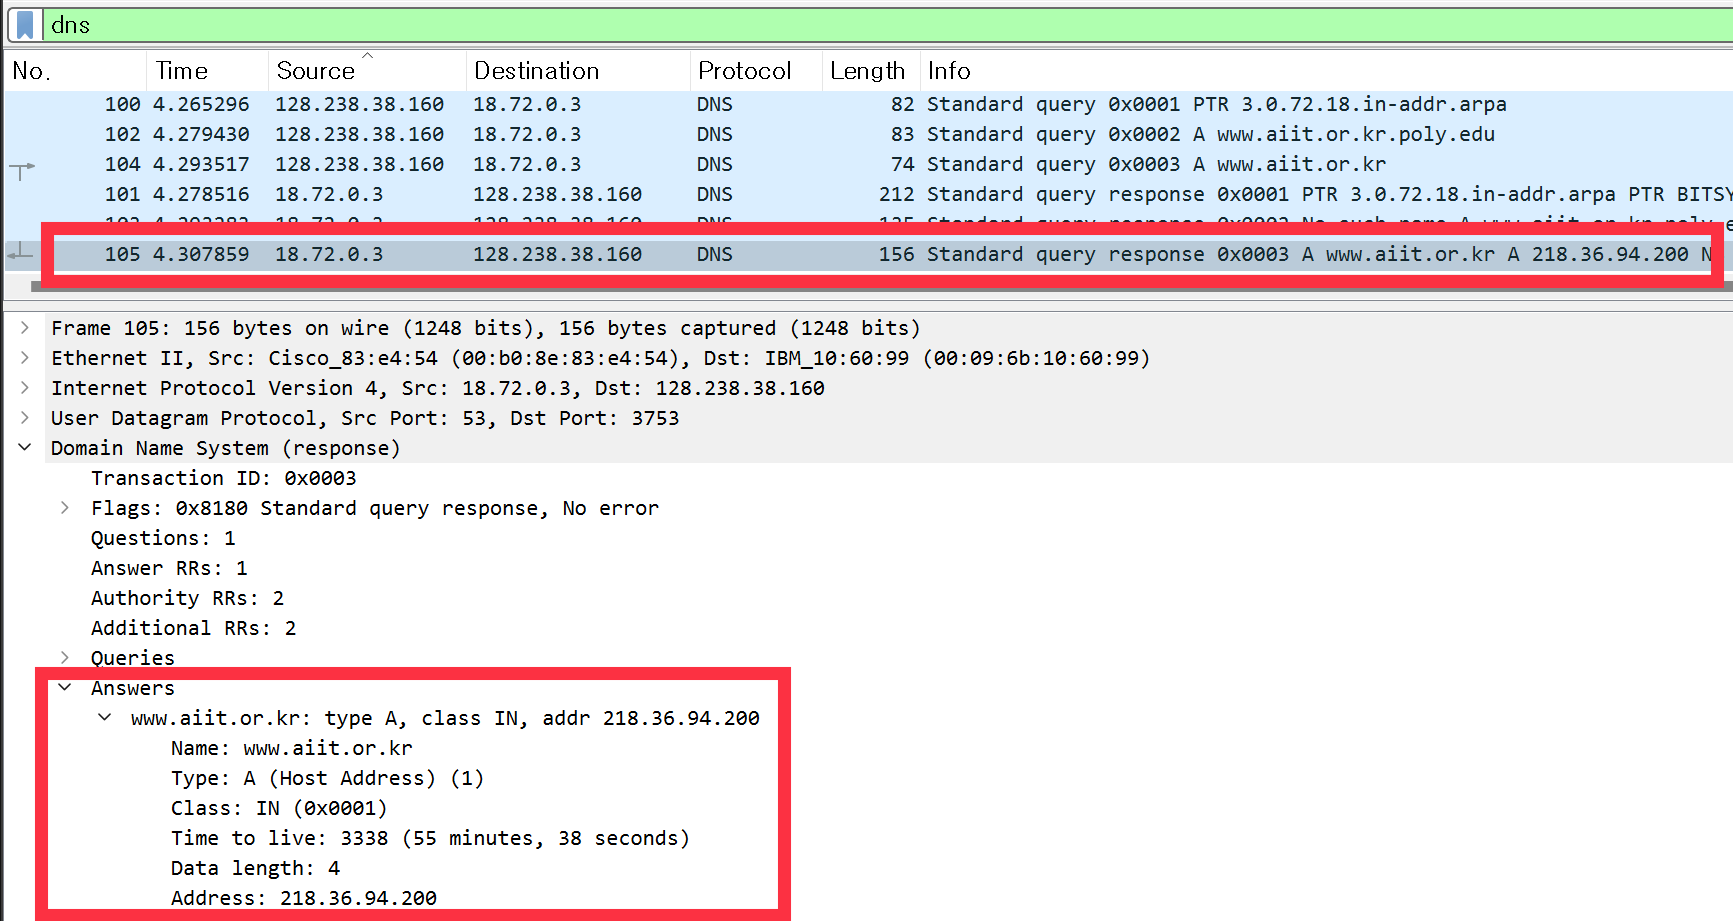
\includegraphics[width=.79\textwidth]{image/result_week01/Q3-h-2.png}
        		\caption{\footnotesize Problem 3-17-2's screenshot : DNS response message, answers}
        		\vspace{-10pt}
            \end{figure}
    \end{enumerate}